\documentclass[a4paper,oneside,10pt]{book}
\usepackage[english]{babel}
\usepackage[portrait,a4paper,margin=2.0cm,headsep=5mm]{geometry}
\usepackage[utf8]{inputenc}
\usepackage[T1]{fontenc}
\usepackage{lmodern}
\usepackage{longtable}
\usepackage[usenames,dvipsnames]{xcolor}
\usepackage[colorlinks=true, linkcolor=blue, urlcolor=blue]{hyperref}
\hypersetup{hidelinks}
\usepackage{array}
\usepackage{graphicx}
\usepackage[labelfont=bf,singlelinecheck=false,format=plain,,justification=justified,indention=0cm]{caption}
\usepackage{listings}
\usepackage{mdframed}

% see ftp://ftp.tex.ac.uk/tex-archive/macros/latex/contrib/listings/listings.pdf

\definecolor{background}{RGB}{255,255,255}
\definecolor{hellgelb}{rgb}{1,1,0.8}
\definecolor{colKeys}{RGB}{127,0,85}
\definecolor{colIdentifier}{rgb}{0,0,0}
\definecolor{colComments}{RGB}{63,127,95}
\definecolor{colString}{RGB}{42,0,255}

% for all listings
\lstset{%
    float=hbp,%
    basicstyle=\ttfamily\small, %
    identifierstyle=\color{colIdentifier}, %
    keywordstyle=\color{colKeys}\bf, %
    stringstyle=\color{colString}, %
    commentstyle=\color{colComments}, %
    columns=flexible, %
    tabsize=2, %
    frame=none, %
    extendedchars=true, %
    showspaces=false, %
    showstringspaces=false, %
    numbers=left, %
    numberstyle=\tiny, %
    breaklines=true, %
    backgroundcolor=\color{background}, %
    breakautoindent=true, %
    captionpos=b%
}

\lstdefinelanguage{ROOM}
{morekeywords={
	handle,
	usercode,
	external,
	outgoing,
	ChoicePoint,
	of,
	semantics,
	initial,
	Attribute,
	import,
	SPP,
	Binding,
	ExitPoint,
	or,
	exit,
	Port,
	ptReal,
	usercode3,
	incoming,
	usercode2,
	usercode1,
	ExternalType,
	SubSystemRef,
	cond,
	conjugated,
	private,
	PrimitiveType,
	SAP,
	PortClass,
	SubSystemClass,
	DataClass,
	sync,
	ActorClass,
	guard,
	ptCharacter,
	ptInteger,
	do,
	LayerConnection,
	TransitionPoint,
	Message,
	relay_sap,
	void,
	LogicalSystem,
	my,
	CompoundProtocolClass,
	ref,
	Behavior,
	ActorInstanceMapping,
	Structure,
	triggers,
	EntryPoint,
	Operation,
	SubProtocol,
	action,
	RefinedState,
	extends,
	conjugate,
	and,
	Interface,
	default,
	cp,
	StateMachine,
	satisfied_by,
	Transition,
	ptBoolean,
	sub,
	model,
	from,
	sends,
	RoomModel,
	ActorRef,
	RefinedTransition,
	LogicalThread,
	ServiceImplementation,
	ProtocolClass,
	abstract,
	regular,
	in,
	async,
	subgraph,
	State,
	entry,
	datadriven,
	eventdriven,
	out,
	handler,
	AnnotationType,
	optional,
	mandatory,
	attribute,
	ActorBehavior,
	target,
	Enumeration,
}
sensitive=false,
morecomment=[l]{//},
morecomment=[s]{/*}{*/},
morestring=[b]",
} 


\lstdefinelanguage{Config}
{morekeywords={
	polling,
	timer,
	ms,
	model,
	Attr,
	file,
	path,
	from,
	InterfaceItem,
	ActorClassConfig,
	write,
	false,
	read,
	import,
	min,
	max,
	ProtocolClassConfig,
	regular,
	true,
	ActorInstanceConfig,
	conjugate,
	dynamic,
	configuration,
	Port,
	SubSystemConfig,
	ConfigModel,
	user,
	import,
	user,
	constructor,
}
sensitive=false,
morecomment=[l]{//},
morecomment=[s]{/*}{*/},
morestring=[b]",
} 

\lstdefinelanguage{etPhys}
{morekeywords={
	ns,
	NodeRef,
	model,
	interval,
	RuntimeClass,
	singleThreaded,
	runtime,
	from,
	multiThreaded,
	DefaultThread,
	msgpoolsize,
	execmode,
	mixed,
	blocked,
	import,
	msgblocksize,
	Thread,
	priomin,
	polled,
	PhysicalSystem,
	ms,
	PhysicalModel,
	us,
	stacksize,
	NodeClass,
	priomax,
	prio,
}
sensitive=false,
morecomment=[l]{//},
morecomment=[s]{/*}{*/},
morestring=[b]",
} 

\lstdefinelanguage{etMap}
{morekeywords={
	model,
	MappingModel,
	SubSystemMapping,
	import,
	from,
	Mapping,
	ThreadMapping,
}
sensitive=false,
morecomment=[l]{//},
morecomment=[s]{/*}{*/},
morestring=[b]",
} 

\lstdefinelanguage{PlainText}
{morekeywords={
}
sensitive=false,
morecomment=[l]{//},
morecomment=[s]{/*}{*/},
morestring=[b]",
} 


\setlength{\parindent}{0pt}  
\setlength{\parskip}{4pt plus 1pt minus 0pt}  % Abstand zwischen Absaetzen
 \nonfrenchspacing
 \sloppy

\newcommand{\specialcell}[2][c]{%
  \begin{tabular}[#1]{@{}c@{}}#2\end{tabular}}

% the robust command prevents premature macro expansion
% but the entry in the PDF structure is wrong (redblueTrice)
%\DeclareRobustCommand{\eTrice}{{\color{blue}e}{\color{red}Trice}{}}

% defining these colors fixes a problem with the plain newcommand
% but still the PDF structure entries are wrong (reblueTrice)
\definecolor{RED}{RGB}{255,0,0}
\definecolor{BLUE}{RGB}{0,0,255}
\newcommand{\eTrice}{{\color{blue}e}{\color{red}Trice}{}}

% the following command makes eTrice vanish completely from the PDF structure
%\usepackage{etoolbox}
%\newrobustcmd{\eTrice}{{\color{blue}e}{\color{red}Trice}{}}

\newcommand{\myparagraph}[1]{\paragraph{#1}\mbox{}\\}
%\newcommand{\room}[1]{\textcolor{RedViolet}{\texttt{#1}}}
\newcommand{\room}[1]{\textcolor{Fuchsia}{\textbf{#1}}}
\renewcommand{\familydefault}{\sfdefault}
 
\title{\Huge \eTrice}
\author{\eTrice{} committers and contributors}
\begin{document}

\maketitle

\tableofcontents

\chapter{Introduction}

\section{\eTrice{} Overview}

\subsection{What is \eTrice{}?}

\eTrice{} provides an implementation of the ROOM modeling language (Real Time Object Oriented Modeling) 
together with editors, code generators for Java, C++ and C code and exemplary target middleware.

The model is defined in textual form (Xtext) with graphical editors (Graphiti) for the structural and 
behavioral (i.e. state machine) parts.

\subsection{Reduction of Complexity}

\eTrice{} is all about the reduction of complexity:

\begin{itemize}
\item structural complexity
	\begin{itemize}
	\item by explicit modeling of hierarchical Actor containment, layering and inheritance
	\end{itemize}
\item behavioral complexity
	\begin{itemize}
	\item by hierarchical state machines with inheritance
	\end{itemize}
\item team work complexity
	\begin{itemize}
	\item because loosely coupled Actors provide a natural way to structure team work
	\item since textual model notation allows simple branching and merging
	\end{itemize}
\item complexity of concurrent \& distributed systems
	\begin{itemize}
	\item because loosely coupled Actors are deployable to threads, processes, nodes
	\end{itemize}
\item complexity of variant handling and reuse (e.g. for product lines)
	\begin{itemize}
	\item by composition of existing Actors to new structures
	\item since Protocols and Ports make Actors replaceable
	\item by inheritance for structure, behavior and Protocols
	\item by making use of model level libraries 
	\end{itemize}
\item complexity of debugging
	\begin{itemize}
	\item model level debugging: state machine animation, data inspection and manipulation, message injection, 
	generated message sequence charts
	\item model checking easier for model than for code (detect errors before they occur)
	\end{itemize}
\end{itemize}

\section{Introduction to the ROOM Language}

\subsection{Scope of ROOM}

This chapter will give a rough overview of what ROOM (\textbf{R}eal-time
\textbf{O}bject-\textbf{O}riented \textbf{M}odeling) is and what it is good for.
It will try to answer the following questions:

\begin{itemize}
\item Where does it come from?
\item Which kind of SW-Systems will be addressed?
\item What is the relation between object oriented programming and ROOM?
\item What are the benefits of ROOM?
\item Which consequences must be taken into account?
\end{itemize}

\subsubsection{Where does it come from?}

ROOM was developed in the 1990th on the background of the upcoming mobile applications with the goal to
manage the complexity of such huge SW-Systems. From the very beginning ROOM has focused on a certain type
of SW-Systems and is, in contrast to the UML, well suited for this kind of systems. In this sense, ROOM is
a DSL (Domain Specific Language) for distributed, event driven, real time systems. 

Bran Selic, Garth Gullekson and Paul T. Ward have published the concepts 1994 in the book
\textbf{Real-Time Object-Oriented Modeling}. The company \textit{ObjecTime}\texttrademark{}
developed a ROOM tool which was taken over by \textit{Rational SW}\texttrademark{} and later
on by \textit{IBM}\texttrademark.
The company \textit{Protos Software GmbH}\texttrademark{} also developed a ROOM tool called
\textit{Trice}\texttrademark{} for control software for production machines and automotive systems.
\textit{Trice}\texttrademark{} is the predecessor of \eTrice{} (see Introduction to \eTrice{}). 
 
From our point of view ROOM provides still the clearest, simplest, most complete and best suited modeling
concepts for the real time domain. All later proposals like the UML do not fit as well to this kind of problems.
 

\subsubsection{Which kind of SW-Systems will be addressed?}

As mentioned before ROOM addresses distributed, event driven, real time systems.
But what is a \emph{real time system}? ROOM defines a set of properties
which are typical for a real time system. These properties are:

\begin{itemize}
\item Timeliness
\item Dynamic internal structure
\item Reactiveness
\item Concurrency
\item Distribution
\item Reliability
\end{itemize}

Each of these properties has potential to make SW development complex. If a given system can be characterized
with a combination of or all of these properties, ROOM might be applied to such a system.  

As an example take a look at a washing machine. The system has to react to user interactions, has to handle
some error conditions like a closed water tap or a defective lye pump. It has to react simultaneously to all these inputs.
It has to close the water valve within a certain time to avoid flooding the basement. 
So, the system can be characterized as timely, concurrent and reactive. As long as the washing machine does
not transform to a laundry drier by itself, the system has no dynamic internal structure and as long as all functions
are running on a single micro controller the (SW)-system is not distributed. 
ROOM fits perfect to such a system.

A SW system which mainly consists of data transformations like signal/image processing or a loop controller
(e.g. a PID controller) cannot be characterized with any of the above mentioned properties. However, in the real
world most of the SW systems will be a combination of both. ROOM can be combined with such systems, so that for
example an actor provides a \emph{run to completion} context for calculating an image processing algorithm or a
PID controller.  

\subsubsection{What is the relation between OOP and ROOM?}

The relation between classical object oriented programming and ROOM is comparable to the relation between assembler
programming and C programming. It provides a shift of the object paradigm. The classical object
paradigm provides some kind of information hiding. Attributes can be accessed via access methods. Logical higher level
methods provide the requested behavior to the user.

But as the figure illustrates, the classical object paradigm does not care about concurrency issues. The threads of
control will be provided by the underlying operating system and the user is responsible to avoid access violations
by using those operating system mechanisms directly (semaphore, mutex).

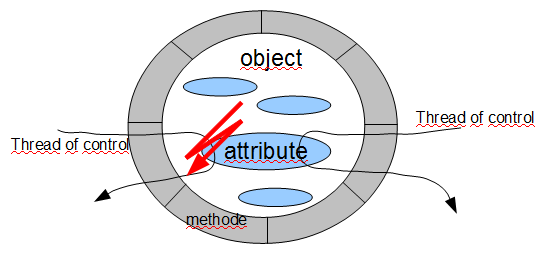
\includegraphics[width=0.6\textwidth]{images/010-RoomIntroduction02.png}

ROOM provides the concept of a logical machine (called actor) with its own thread of control. It provides some kind
of cooperative communication infrastructure with \emph{run to completion} semantics.
That makes developing of business logic easy and safe (see \ref{sec:basic_concepts} \nameref{sec:basic_concepts}). The logical machine provides an 
encapsulation shell including concurrency issues (see \ref{sec:run_to_completion} \nameref{sec:run_to_completion}). 

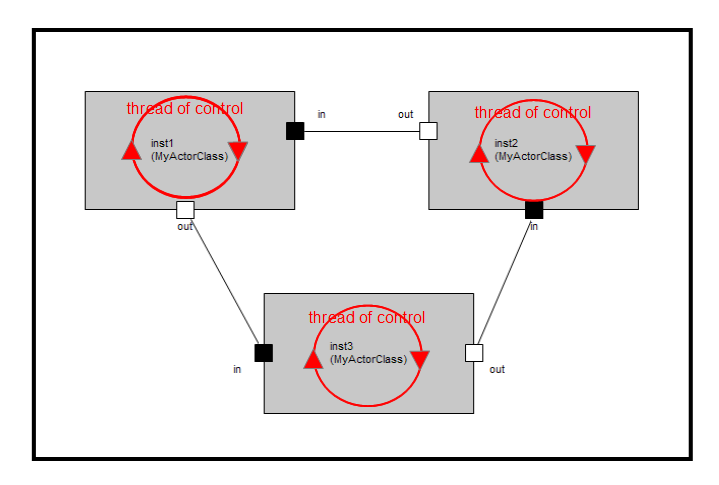
\includegraphics[width=0.8\textwidth]{images/010-RoomIntroduction03.png}

This thinking of an object is much more general than the classic one.  

\subsubsection{What are the benefits of ROOM?}

ROOM has a lot of benefits and it depends on the users point of view which is the most important one. From a general
point of view the most important benefit is, that ROOM allows to create SW systems very efficient, robust and safe
due to the fact that it provides some abstract, high level modeling concepts combined with code generation and a
small efficient runtime environment.  

In detail:
\begin{itemize}
\item ROOM models contain well defined interfaces (protocols), which makes it easy to re-use components in different
applications or e.g. in a test harness. 
\item Graphical modeling makes it easy to understand, maintain and share code with other developers
\item Higher abstraction in combination with automated code generation provides very efficient mechanisms to
the developer. 
\item ROOM provides graphical model execution, which makes it easy to understand the application or find defects in
a very early phase. 
\end{itemize}

\subsubsection{Which consequences must be taken into account?}

Generating code from models will introduce some overhead in terms of memory footprint as well as performance.
For most systems the overhead will be negligible. However, the decision for using ROOM should be made explicitly
and it is always a trade off between development costs, time to market and costs in terms of a little bit more of
memory and performance. Thanks to the powerful component model, ROOM is especially well suited for the development
of software product lines with their need for reusable core assets.  
  
Care must be taken during the introduction of the new methodology. Due to the fact that ROOM provides a shift of the
object paradigm, developers and teams need a phase of adaption. Every benefit comes at a price.

\subsection{Basic Concepts}
\label{sec:basic_concepts}

\subsubsection{Actor, Port, Protocol}

The basic elements of ROOM are the actors with their ports and protocols.
The protocol provides a formal interface description. The port is an interaction
point where the actor interacts with its outside world. Each port has exactly one protocol
attached. The sum of all ports builds up the complete interface of an actor.
Each port can receive messages, with or without data, which are defined in the attached protocol.
Each message will be handled by the actor's behavior (state machine) or will be delegated to the actor's internal structure.

\begin{table}
\caption{Actor and Protocol Class Example}
\begin{tabular}{|l|l|}
\hline
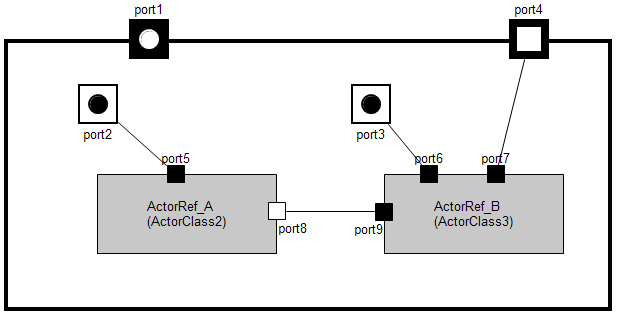
\includegraphics[scale=0.85]{images/040-ActorClass.png} & 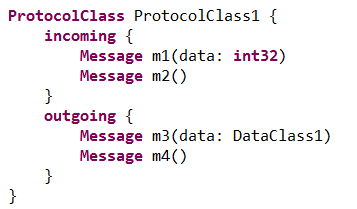
\includegraphics[scale=0.85]{images/040-ProtocolClassTextualNotation.png} \\ \hline
\textbf{Actor with sub actors} & \textbf{Protocol definition} \\ \hline
\end{tabular}
\end{table}

The actor provides access protection for its own attributes (including complex types, i.e. classical objects), 
including concurrency protection. An actor has neither public attributes nor public operations. The only 
interaction with the outside world takes place via interface ports. This ensures a high degree of 
re-usability on the actor level and provides an effective and safe programming model to the developer. 

Receiving a message via a port will trigger the internal state machine. A transition will be executed 
depending on the message and the current state. Within this transition, detail level code will be executed 
and response messages can be sent.

With this model, a complex behavior can be divided into many relatively simple, linked actors. To put it the 
other way round: The complex behavior will be provided by a network of relatively simple components which 
are communicating with each other via well defined interfaces.


\subsubsection{Hierarchy in Structure and Behavior}

ROOM provides two types of hierarchy. Behavioral hierarchy and structural hierarchy. Structural hierarchy 
means that actors can be nested to arbitrary depth. Usually you will add more and more details to your 
application with each nesting level. That means you can focus yourself on any level of abstraction with 
always the same element, the actor. Structural hierarchy provides a powerful mechanism to divide your 
problem in smaller pieces, so that you can focus on the level of abstraction you want to work on. 

The actor's behavior will be described with a state machine. A state in turn may contain sub states. This 
is another possibility to focus on an abstraction level. Take the simple FSM from the blinky actor from 
the blinky tutorial. 
   
Top level:

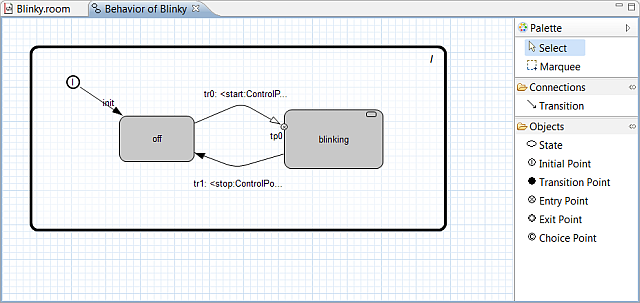
\includegraphics[width=0.8\textwidth]{images/020-Blinky15.png}

\textit{blinking} Sub machine:

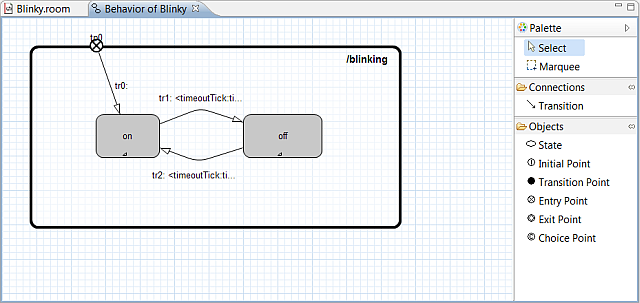
\includegraphics[width=0.8\textwidth]{images/020-Blinky151.png}

From an abstract point of view there is a state \textit{blinking}. But a simple LED is not able to blink 
autonomously. Therefore you have to add more details to your model to make a LED blinking, but for the 
current work it is not of interest how the blinking is realized. This will be done in the next lower level 
of the hierarchy. 

This simple example might give an idea how powerful this mechanisms is.

The hierarchical FSM provides a rich tool box to describe real world problems (see chapter \ref{sec:room_concepts} \nameref{sec:room_concepts}).

\subsubsection{Layering}

Layering is another well known form of abstraction to reduce complexity in the structure of systems. ROOM 
is probably the only language that supports layering directly as a language feature.
Layering can be expressed in ROOM by actors with specialized ports, called \emph{Service Access Points} 
(SAP) and \emph{Service Provision Points} (SPP).

The actor that provides a service implements an SPP and the client of that service implements an SAP. The 
layer connection connects all SAPs of a specific protocol within an actor hierarchy with an SPP that 
implements the service. From the actor's point of view, SAPs and SPPs behave almost like ports.

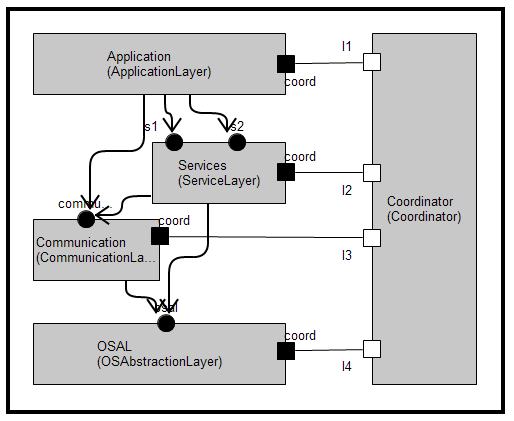
\includegraphics{images/010-LayerExample.png}

The example shows a layered model. The layer connections define e.g. that the \textit{ApplicationLayer} 
can only use the services of the \textit{ServiceLayer} and the \textit{CommunicationLayer}. Actors inside 
the \textit{ApplicationLayer} that implement an SAP for those services are connected directly to the 
implementation of the services. 
Layering and actor hierarchies with port to port connections can be mixed on every level of granularity. 

\subsubsection{Run to Completion}
\label{sec:run_to_completion}

\emph{Run to completion} (RTC) is a very central concept of ROOM. It enables the developer to 
concentrate on the functional aspects of the system. The developer doesn't have to care about concurrency 
issues all the time. This job is concentrated to the system designer in a very flexible way.
What does \emph{run to completion} mean:
RTC means that an actor, which is processing a message, can not receive the next message as long as the 
processing of the current message has been finished. Receiving of the next message will be queued by the 
underlying run time system.

Note: It is very important not to confuse \emph{run to completion} and \emph{cooperative multi threading}.
Run to completion means that 
an actor will finish the processing of a message before he can receive a new one (regardless of its 
priority). That does \emph{not} mean that an actor cannot be preempted from an higher priority thread of control. 
But even a message from this higher prior thread of control will be queued until the current processing 
has been finished. 

With this mechanism all actor internal attributes and data structures are protected. Due to the fact that 
multiple actors share one thread of control, all objects are protected which are accessed from one thread 
of control but multiple actors. This provides the possibility to decompose complex functionality into 
several actors without the risk to produce access violations or dead locks.

\subsection{Execution Models}

Since from ROOM models executable code can be generated, it is important to define the way the actors are 
executed and communicate with each other. The combination of communication and execution is called the 
\emph{execution model}.
Currently the \eTrice{} tooling supports the \textbf{message driven}, the \textbf{data 
driven} and a mixture of both execution models. In future releases maybe also a synchronous
execution model will be supported, depending on the 
requirements of the community.

\subsubsection{Communication Methods}

\begin{itemize}
\item \textbf{message driven} -- asynchronous, non blocking, no return value:\\
Usually the message driven 
communication is implemented with message queues. Message queues are inherently asynchronous and enable a 
very good decoupling of the communicating parties.
\item \textbf{data driven} -- asynchronous, non blocking, no return value:\\
In data driven communication 
sender and receiver often have a shared block of data. The sender writes the data and the receiver polls 
the data.
\item \textbf{function call} -- synchronous, blocking, return value:\\
Regular function call as known in most 
programming languages.
\end{itemize}

\eTrice{} currently supports the two former communication methods.

\subsubsection{Execution Methods}

\begin{itemize}
\item \textbf{execution by receive event}: The message queue or the event dispatcher calls a 
\textbf{receive event} function of the message receiver and thereby executes the processing of the event.
\item \textbf{polled execution}: The objects are processed by a cyclic \textbf{execute} call
\item \textbf{execution by function call}: The caller executes the called object via function call
\end{itemize}

\eTrice{} currently supports the two former execution methods.

\subsubsection{Execution Models}

In present-day's embedded systems in most cases one or several of the following execution models are used:

\myparagraph{message driven}

The message driven execution model is a combination of message driven communication and execution by 
receive event.
This model allows for distributed systems with a very high throughput.
It can be deterministic but the determinism is hard to proof.
This execution model is often found in telecommunication systems and high performance automation control 
systems.

\myparagraph{data driven}

The data driven execution model is a combination of data driven communication and polled execution.
This model is highly deterministic and very robust, but the polling creates a huge performance overhead.
The determinism is easy to proof (simple mathematics). 
The execution model is also compatible with the execution model of control software generated by Tools 
like Matlab(TM) and LabView(TM).
This model is usually used for systems with requirements for safety, such as automotive and avionic systems.

\myparagraph{synchronous}

The synchronous execution model could also be called \emph{function calls}. 
This model in general is not very well suited to support the \emph{run to completion} semantics typical 
for ROOM models, but could also be generated from ROOM models. 
With this execution model also lower levels of a software system, such as device drivers, could be 
generated from ROOM models.


\chapter{Tutorials}

\chapter{Working with the eTrice Tutorials}

The eTrice Tutorials will help you to learn and understand the eTrice tool and concepts. ETrice supports 
several target languages. The concepts will not be explained for each language. 

Most of the common concepts will be described for Java as target language. To start with a new language the 
first steps to setup the workspace and to generate and run the first model will be described also. Target 
language specific aspects will be described as well.

Therefore the best way to start with eTrice is to follow the Java Tutorials and after that switch to your 
target language.  

\section{Setting up the Workspace for Java Projects}

After installation of eclipse and the \eTrice{} plug in, your workspace should look like this:  

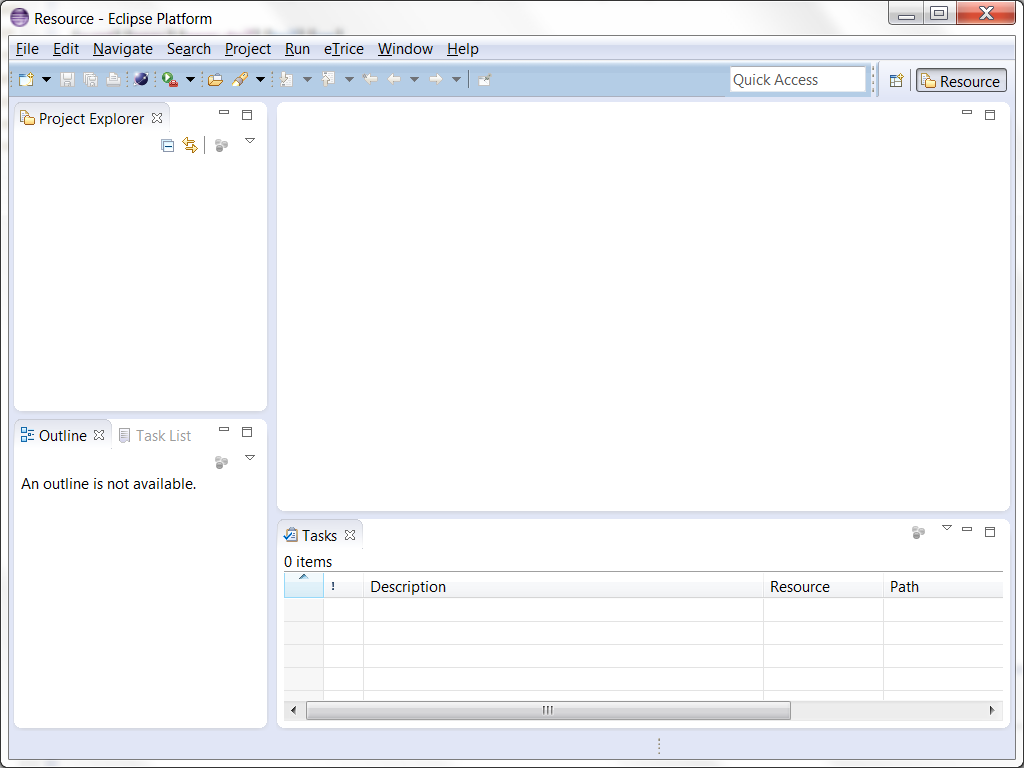
\includegraphics[width=0.8\textwidth]{images/013-SetupWorkspace01.png}
% !images/013-SetupWorkspace01.png!

Just the \textit{\eTrice{}} menu item is visible of the installed \eTrice{} plugins.

Select the menu \textbf{File->New->Other}

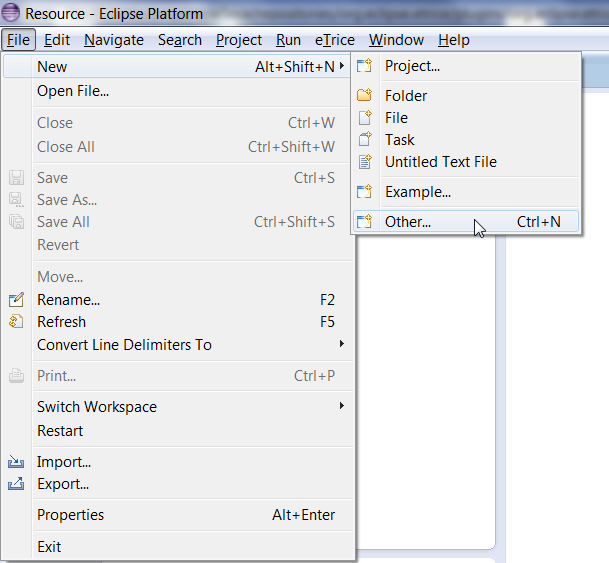
\includegraphics[width=0.8\textwidth]{images/013-SetupWorkspace02.png}
% !images/013-SetupWorkspace02.png!

Open the \textit{\eTrice{}} tab and select \textit{\eTrice{} Java Runtime}

Press \textit{Next} and \textit{Finish} to install the Runtime into your workspace.

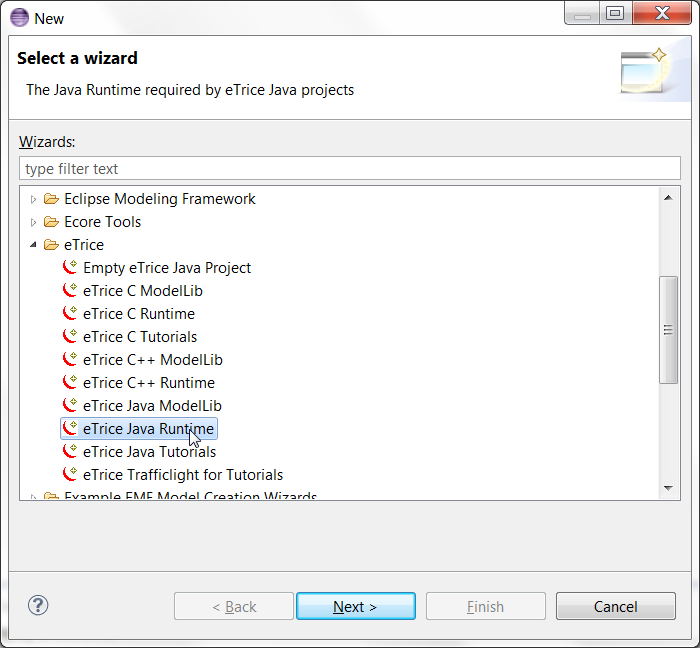
\includegraphics[width=0.8\textwidth]{images/013-SetupWorkspace03.png}
% !images/013-SetupWorkspace03.png!

Do the same steps for \textit{\eTrice{} Java Modellib} and \textit{\eTrice{} Java Tutorials}. To avoid temporary 
error markers you should keep the proposed order of installation. The resulting workspace should look like 
this:

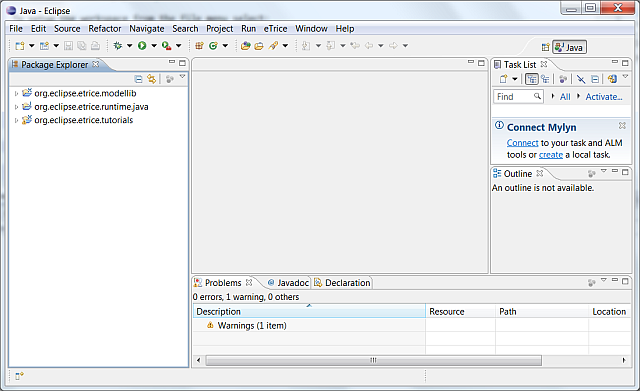
\includegraphics[width=0.8\textwidth]{images/013-SetupWorkspace04.png}
% !images/013-SetupWorkspace04.png!

Now workspace is set up and you can perform the tutorials or start with your work.

The tutorial models are available in the \textit{org.eclipse.etrice.tutorials.java} project. All tutorials are 
ready to generate and run without any changes. To start the code generator simply run 
\textbf{gen\_org.eclipse.etrice.tutorials.java.launch} as \textbf{gen\_org.eclipse.etrice.tutorials.java}: 

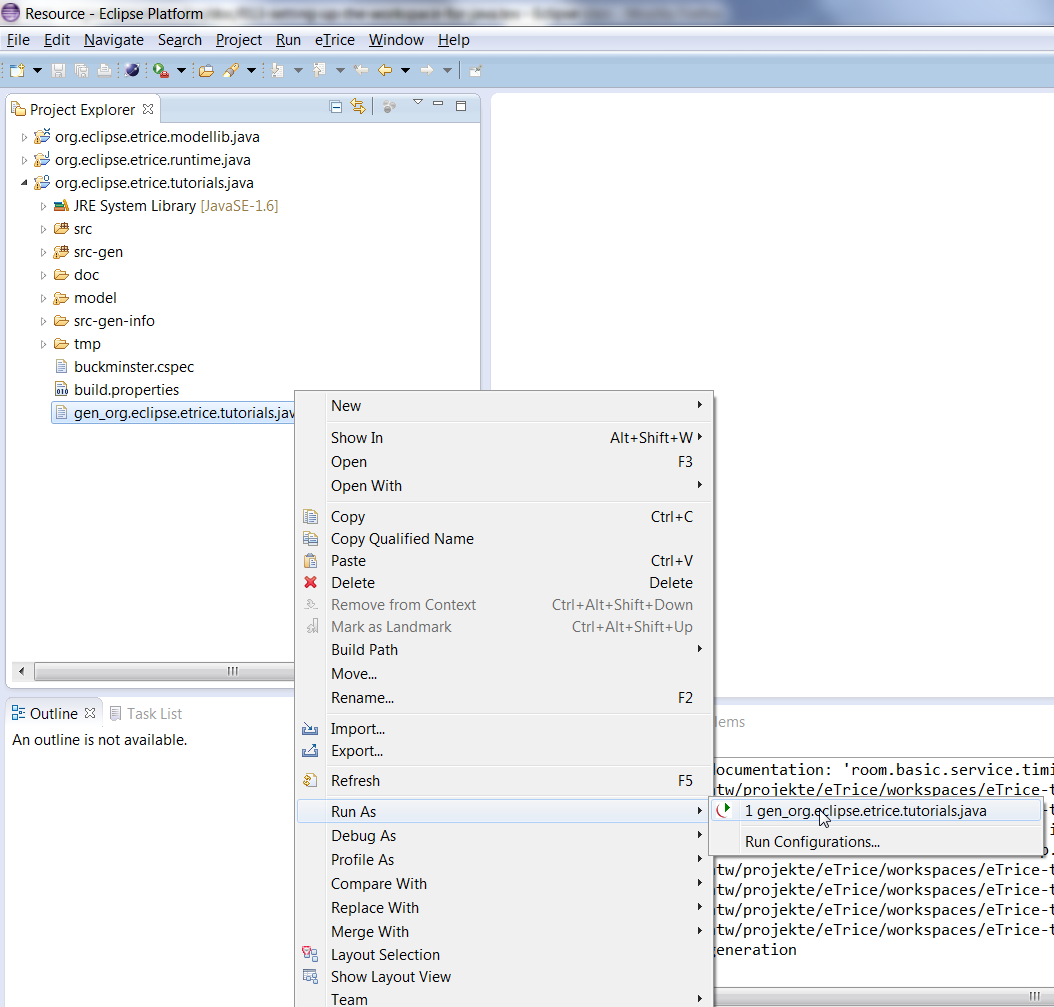
\includegraphics[width=0.8\textwidth]{images/013-SetupWorkspace05.png}
% !images/013-SetupWorkspace05.png!

The successful generation ends with \emph{Info: -- finished code generation} in the Console.

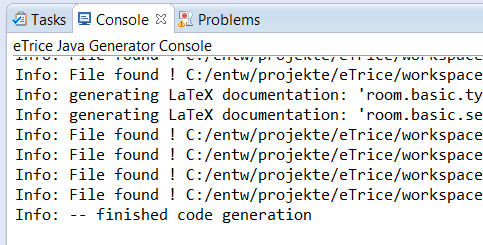
\includegraphics[width=0.8\textwidth]{images/013-SetupWorkspace051.png}
% !images/013-SetupWorkspace051.png!


For each tutorial in the folder src-gen a java package is generated including a java file called 
\textbf{SubSystem\_<Modelname>Runner.java} . To run the a generated application simply run this file as a java application:

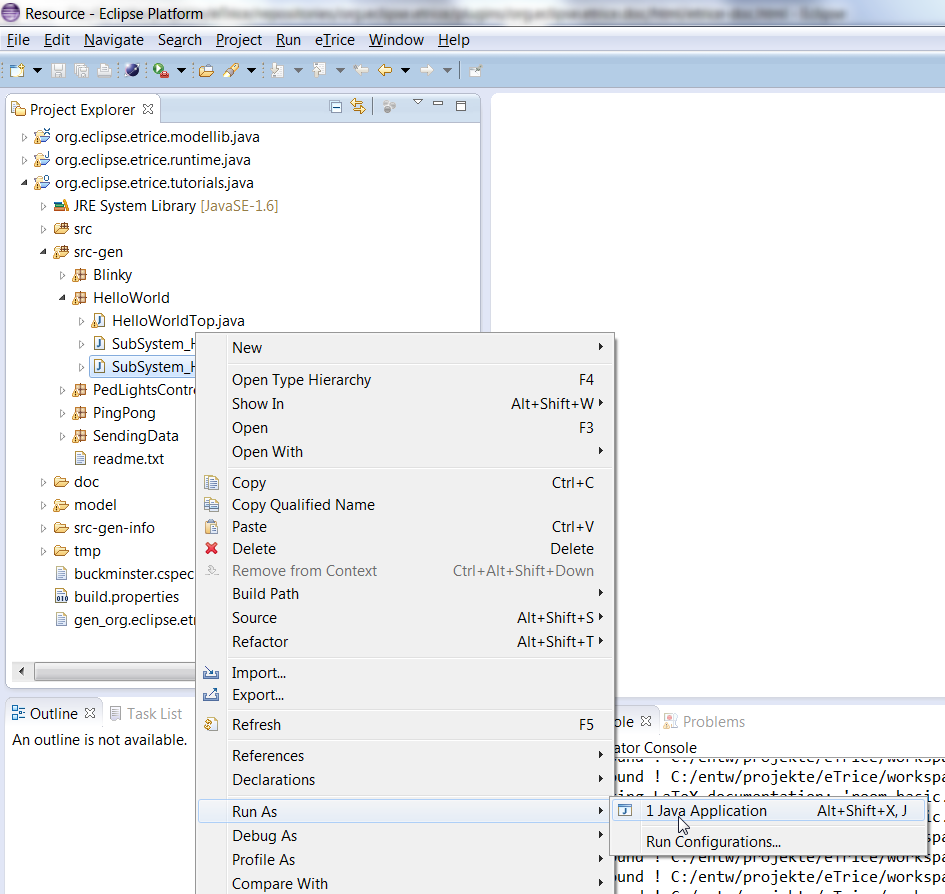
\includegraphics[width=0.8\textwidth]{images/013-SetupWorkspace06.png}
% !images/013-SetupWorkspace06.png!

To stop the application type \textit{quit} in the console window.
 
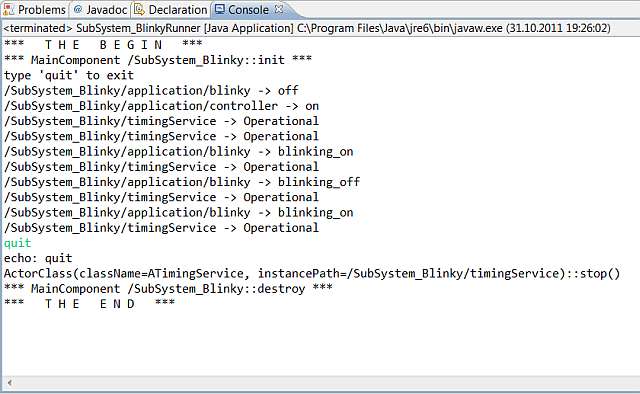
\includegraphics[width=0.8\textwidth]{images/013-SetupWorkspace07.png} 
% !images/013-SetupWorkspace07.png!

Performing the tutorials will setup a dedicated project for each tutorial. Therefore there are some 
slight changes especially whenever a path must be set (e.g. to the model library) within your own 
projects. All this is described in the tutorials.

\section{Setting up the Workspace for C Projects}

\textbf{Objectives for this tutorial:}
\begin{itemize}
	\item create all needed library projects (runtime.c and modellib.c)
	\item create the tutorial project with the examples
	\item create the project with a traffic light simulator
	\item test the workspace setup by running one of the examples
\end{itemize}

\subsection{Create Library, Tutorial and Simulator Projects}

Before you can start with C, some preconditions must be fulfilled:

\begin{itemize}
\item A C compiler must be installed on your machine. All tutorials are based on MinGW/GCC (Windows) and Posix/GCC (Linux), but currently only tested on Windows with MinGW/GCC
\item The CDT-Eclipse plugin must be installed as the C development environment.
\end{itemize}

After installation of eclipse and the \eTrice{} plug in, your workspace should look like this:  

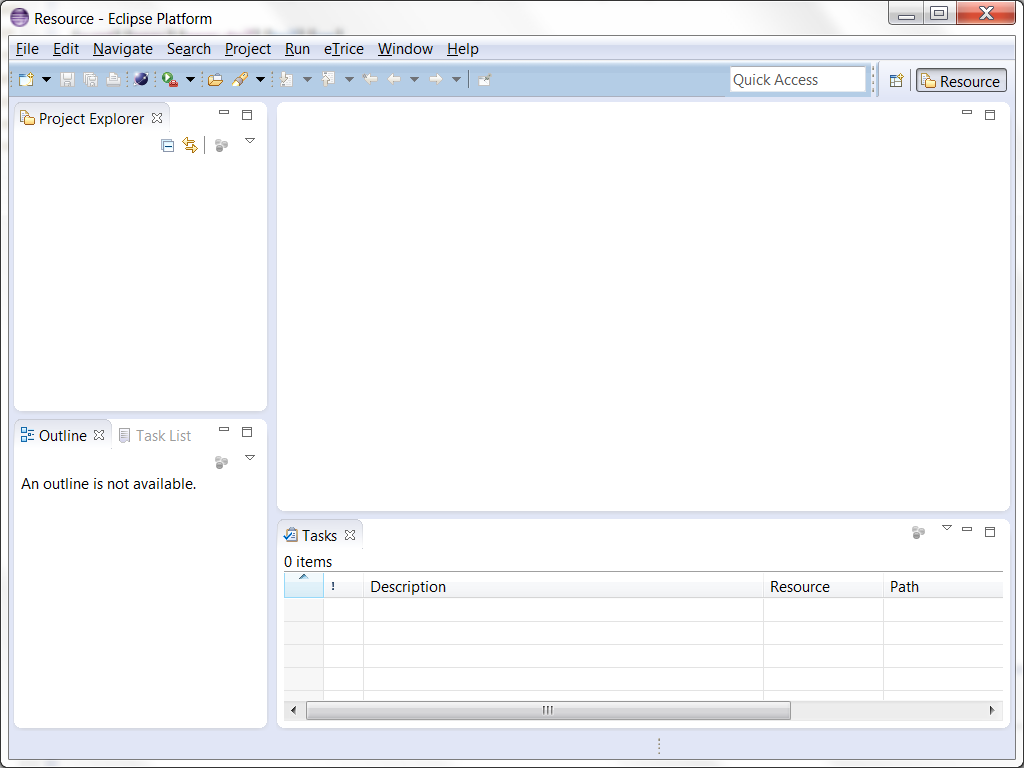
\includegraphics[width=0.8\textwidth]{images/013-SetupWorkspace01.png}
% !images/013-SetupWorkspace01.png!

Just the \eTrice{} menu item is visible of the installed \eTrice{} plugins.

\newpage
Select the menu \emph{File->New->Other}

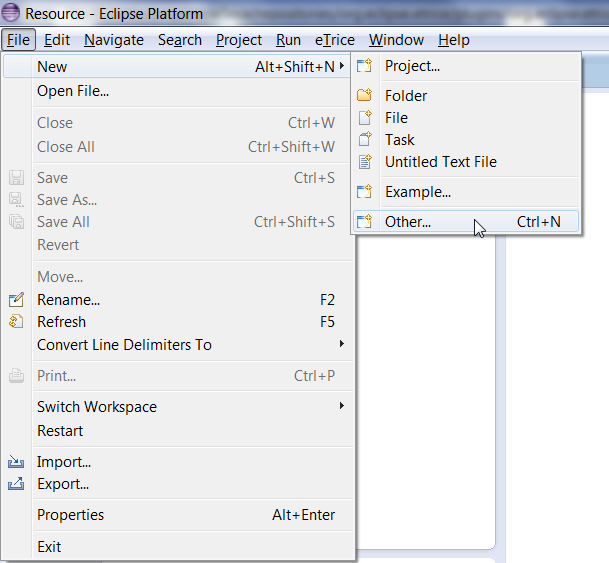
\includegraphics[width=0.6\textwidth]{images/013-SetupWorkspace02.png}
% !images/013-SetupWorkspace02.png!

Open the \emph{eTrice} tab and select \textit{eTrice C Runtime}

Press \emph{Next} and \emph{Finish} to install the Runtime into your workspace.

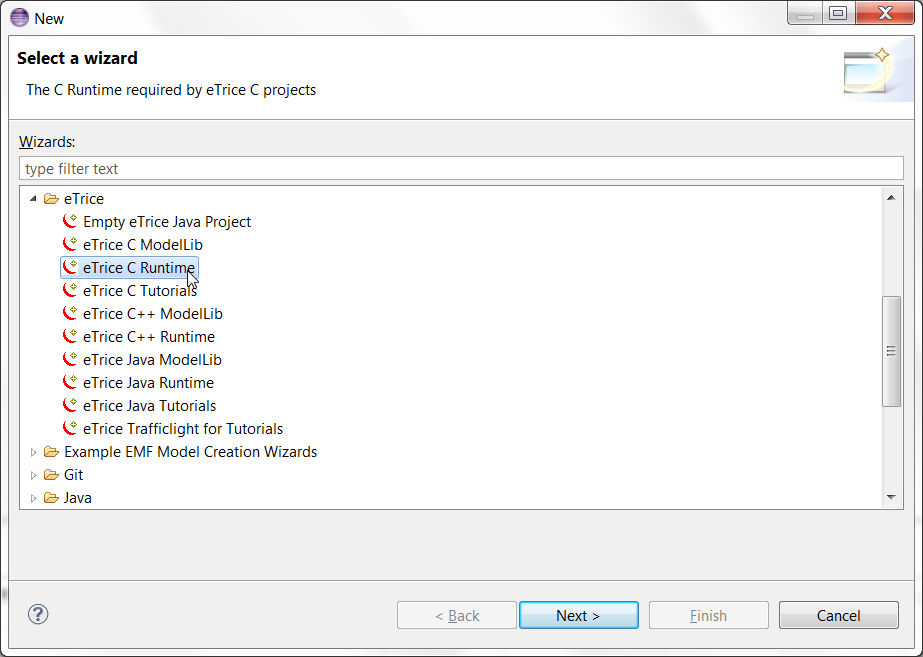
\includegraphics[width=0.6\textwidth]{images/014-SetupWorkspaceC005.png}
% !images/014-SetupWorkspaceC005.png!

\newpage
Do the same steps for \textit{eTrice C Modellib}, \textit{eTrice C Tutorials} and \textit{eTrice Trafficlight for Tutorials}. To avoid temporary 
error markers you should keep the proposed order of installation. The resulting workspace should look like 
this:

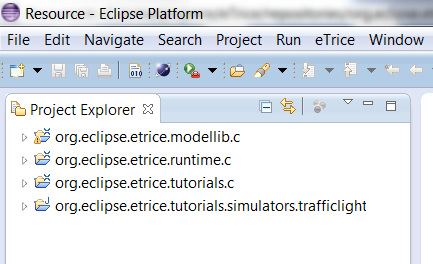
\includegraphics[width=0.5\textwidth]{images/014-SetupWorkspace007.png}
% !images/014-SetupWorkspace007.png!

\subsection{Perform Setup Test}

To check the correct setup of your workspace we run a little testproject contained in the tutorial project.

The tutorial models are available in the  \emph{org.eclipse.etrice.tutorials.c} project. All tutorials are ready to generate and run without any changes. To test the code generator and the workspace setup simply run 
\emph{gen\_SetupTestC.launch} as \emph{gen\_SetupTestC}: 

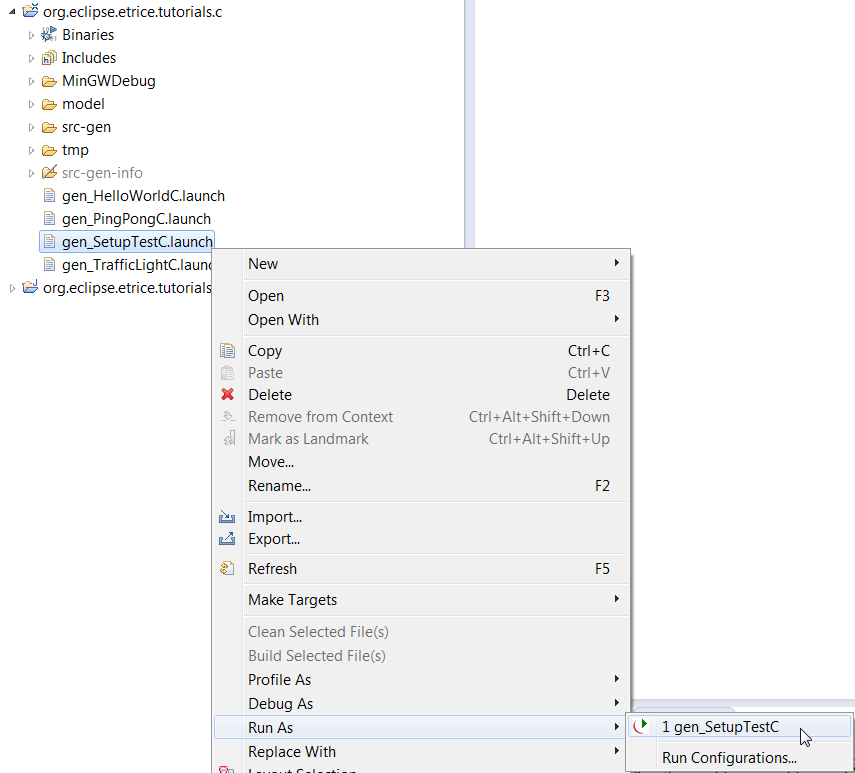
\includegraphics[width=0.6\textwidth]{images/014-05-gen_SetupTestC.png}
% !images/014-05-gen_SetupTestC.png!

\newpage
The successful generation ends with \emph{Info: -- finished code generation} in the Console.

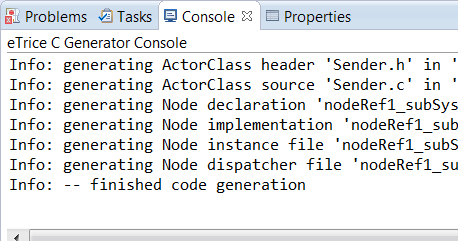
\includegraphics[width=0.5\textwidth]{images/014-06-FinishedCodeGeneration.png}
% !014-06-FinishedCodeGeneration.png!

For each tutorial in the folder src-gen a sub folder is generated which contains the generated code. The file \emph{<...>\_Runner.c} contains the main function. To run the generated application you first have to compile the project (with the hammer symbol in the C/C++ Perspective).

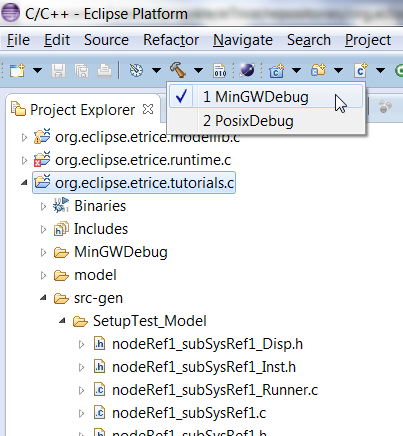
\includegraphics[width=0.5\textwidth]{images/014-07-Compile.png}
% !014-07-Compile.png!

If the compilitation does not succeed, make sure to clean and compile the projects \emph{org.eclipse.etrice.runtime.c} and \emph{org.eclipse.etrice.modellib.c} with the correct build configuration for your platform. Depending on the setup of your C compiler and CDT you might have to change the pre defined build configurations \emph{MinGWDebug} or \emph{PosixDebug}.

After the successful compilation you can run the application as \emph{Local C/C++ Application}.

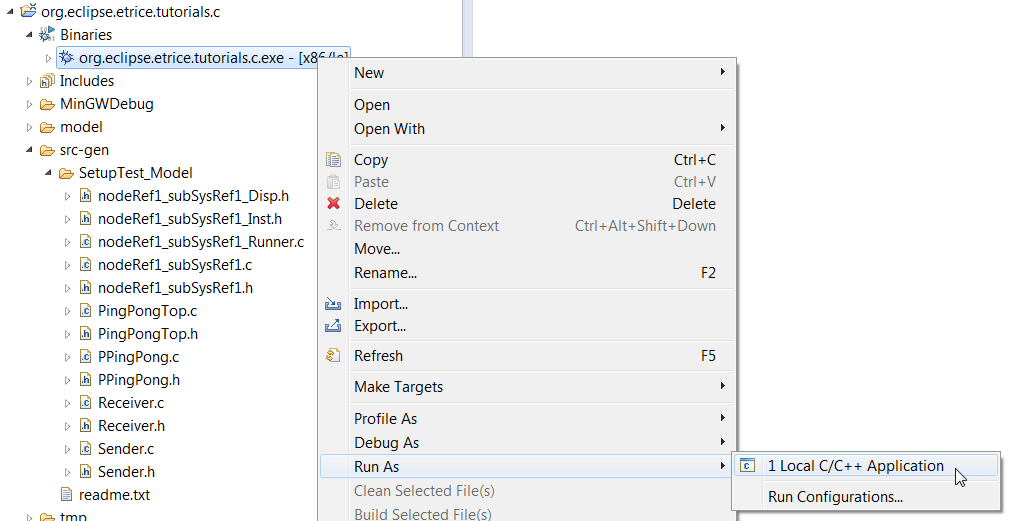
\includegraphics[width=0.7\textwidth]{images/014-08-RunAsC-CPP-Application.png}
% !images/014-08-RunAsC-CPP-Application.png!

\newpage
To stop the application type \emph{quit} in the console window. If your Console contains the lines
\begin{verbatim}
******************
*** Setup OK ***
******************
\end{verbatim}
your setup should be ok.

%TODO : update screenshot
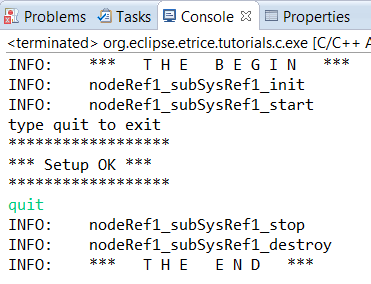
\includegraphics[width=0.5\textwidth]{images/014-09-ConsoleWithSetupOk.png} 
% !images/014-09-ConsoleWithSetupOk.png!

Now the workspace is set up and you can perform the tutorials or start with your work.


\section{HelloWorld for Java}

\subsection{Scope}

In this tutorial you will build your first very simple \eTrice{} model. The goal is to learn the work flow of 
\eTrice{} and to understand a few basic features of ROOM. You will perform the following steps:

\begin{enumerate}
\item create a new model from scratch
\item add a very simple state machine to an actor
\item generate the source code
\item run the model
\item open the message sequence chart
\end{enumerate}

Make sure that you have set up the workspace as described in \emph{Setting up the Workspace for Java}.

\subsection{Create a new model from scratch}

The easiest way to create a new \eTrice{} Project is to use the eclipse project wizard. From the eclipse file 
menu select \emph{File->New->Project} and create a new \emph{Empty eTrice Java Project} and name it \textbf{HelloWorld}.

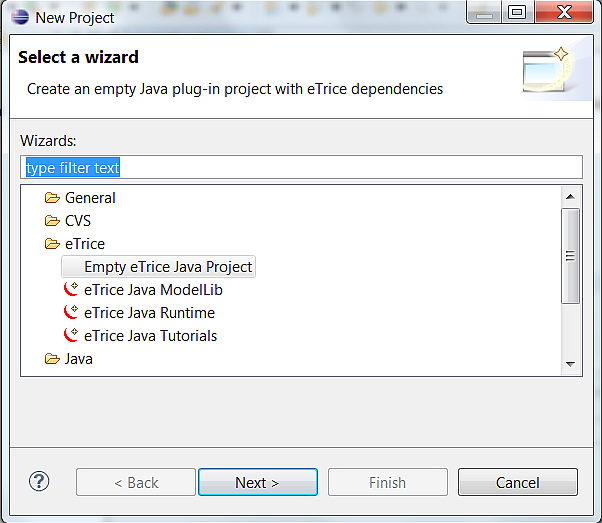
\includegraphics[width=0.8\textwidth]{images/015-HelloWorld10.png}

The wizard creates everything that is needed to create, build and run an \eTrice{} model. The resulting 
project should look like this:

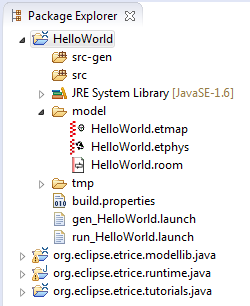
\includegraphics{images/015-HelloWorld11.png}

Within the model directory the model file \emph{HelloWorld.room} was created. Open the 
\emph{HelloWorld.room} file and delete the contents of the file. Open the content assist with Ctrl+Space 
and select \emph{RoomModel - model skeleton}.

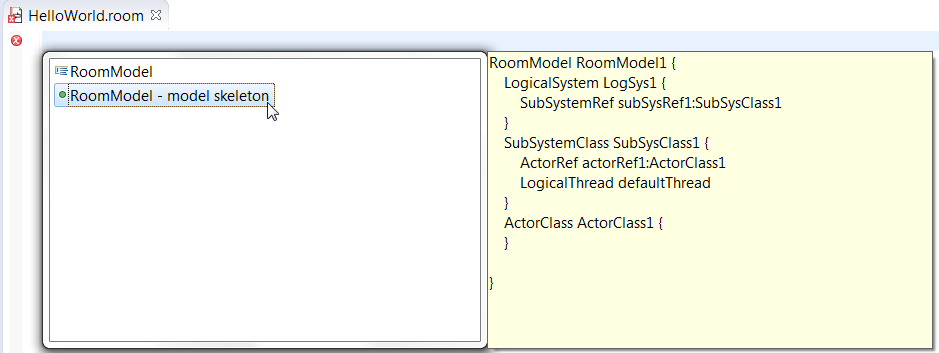
\includegraphics[width=0.6\textwidth]{images/015-HelloWorld12.png}

Edit the template variables by typing the new names and jumping with Tab from name to name.

The resulting model code should look like this:

\begin{lstlisting}[language=ROOM]
RoomModel HelloWorld_Model {

	LogicalSystem LogSys1 {
		SubSystemRef subSysRef1: SubSysClass1
	}

	SubSystemClass SubSysClass1 {
		ActorRef actorRef1: HelloWorldTop
		LogicalThread defaultThread
	}

	ActorClass HelloWorldTop { }

}
\end{lstlisting}

The physical model has already been created for us in file model/HelloWorld.etphys.
We can just leave it as it is.

\begin{lstlisting}[language=etPhys]
PhysicalModel PhysicalModel1 {

	PhysicalSystem PhysSys1 {
		NodeRef nodeRef1 : NodeClass1
	}

	NodeClass NodeClass1 {
		runtime = RuntimeClass1
		priomin = -10
		priomax = 10
		DefaultThread PhysicalThread1 {
			execmode = mixed
			interval = 100 ms
			prio = 0
			stacksize = 1024
			msgblocksize = 32
			msgpoolsize = 10
		}
	}

	RuntimeClass RuntimeClass1 {
		model = multiThreaded
	}
}
\end{lstlisting}

The physical model defines the setup of your nodes with their attributes like threads and mode of execution. In this case we define one node with one thread. 

Similar for the mapping model model/HelloWorld.etmap which is used to deploy the logical system onto the physical system.

\begin{lstlisting}[language=etMap]
MappingModel MappingModel1 {
	import HelloWorld_Model.* from "HelloWorldC.room"
	import PhysicalModel1.* from "HelloWorldC.etphys"
	Mapping LogSys1 -> PhysSys1 {
		SubSystemMapping subSysRef1 -> nodeRef1 {
			ThreadMapping defaultThread -> PhysicalThread1
		}
	}
}
\end{lstlisting}

The goal of \eTrice{} is to describe distributed systems on a logical level. In the current version not all 
elements will be used. But as prerequisite for further versions the following elements can be defined:
\begin{itemize}
\item the \textit{LogicalSystem} (currently optional)
\item at least one \textit{SubSystemClass} (mandatory)
\item at least one \textit{ActorClass} (mandatory)
\end{itemize}

The \textit{LogicalSystem} represents the complete distributed system and contains at least one 
\textit{SubSystemRef}. The \textit{SubSystemClass} represents an address space (e.g. a linux process or an image for a microcontroller) and contains at least one 
\textit{ActorRef}. The \textit{ActorClass} is the building block for building the hierachical structure of an application. 
A good point to start is to define a top level actor that can be used as structural root within the subsystem.

The outline view of the textual ROOM editor shows the main modeling elements in a navigation tree. You can jump to an element in the textual editor by double clicking the element in the outline view.

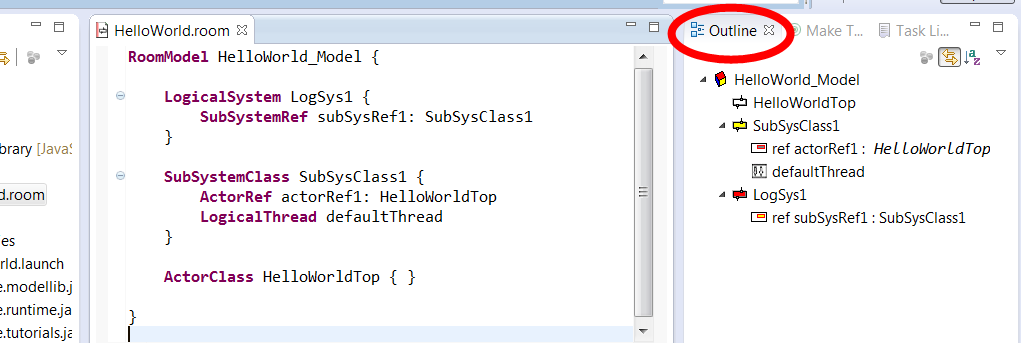
\includegraphics[width=0.8\textwidth]{images/015-HelloWorld02.png}
% !images/015-HelloWorld02.png!

\subsection{Create a state machine}

We will implement the Hello World code on the initial transition of the \textit{HelloWorldTop} actor. 
Therefore open the state machine editor by right clicking the \textit{HelloWorldTop} actor in the outline view and select \textit{Edit Behavior}.

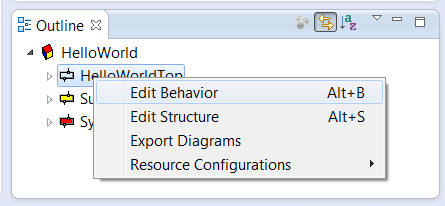
\includegraphics{images/015-HelloWorld03.png}
% !images/015-HelloWorld03.png!

The state machine editor will be opened. Drag and drop an \textit{Initial Point} from the tool box to the 
diagram into the top level state. Drag and drop a \textit{State} from the tool box to the diagram. Confirm the dialogue with \textit{ok}. Select the \textit{Transition} in the tool box and draw the transition from the \textit{Initial Point} to the State. Open the transition dialogue by double clicking the transition arrow and fill in the action code. Be aware of the different action code in Java and C.

\begin{figure}[ht]
\begin{minipage}[b]{0.45\linewidth}
	\begin{mdframed}
	\textbf{action code for Java}
	\begin{verbatim}
	System.out.println("Hello World !");
	\end{verbatim}
	\end{mdframed}
\end{minipage}
\hspace{0.5cm}
\begin{minipage}[b]{0.45\linewidth}
	\begin{mdframed}
	\textbf{action code for C}
	\begin{verbatim}
	printf("Hello World\n");
	\end{verbatim}
	\end{mdframed}
\end{minipage}
\end{figure}

 
The result should look like this:

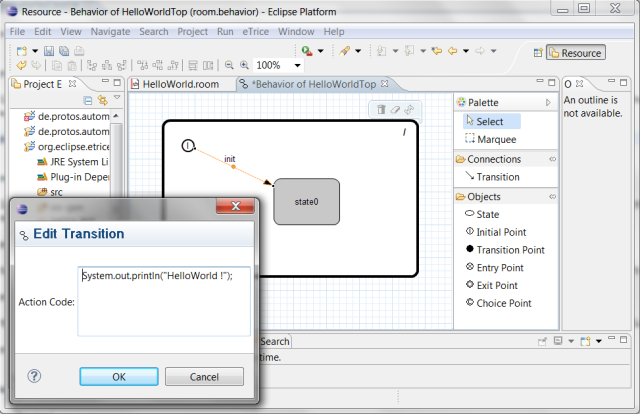
\includegraphics[width=0.8\textwidth]{images/015-HelloWorld04.png}
% !images/015-HelloWorld04.png!

Save the diagram and inspect the model (HelloWorld.room) file. Note that the textual representation was changed after saving 
the diagram.

\begin{figure}[ht]
\begin{minipage}[t]{0.50\linewidth}
\begin{mdframed}
	\textbf{room model for Java}
	\newline
\begin{lstlisting}[language=ROOM]
RoomModel HelloWorld_Model {
	LogicalSystem LogSys1 {
		SubSystemRef subSysRef1:SubSysClass1 
	}
	SubSystemClass SubSysClass1 {
		ActorRef actorRef1:HelloWorldTop 
		LogicalThread defaultThread
	}
	ActorClass HelloWorldTop {
		Structure { }
		Behavior {
			StateMachine {
				Transition init: initial -> state0 {
					action {
						"System.out.println(\"Hello World\");"
					}
				}
				State state0
			}
		}
	}
}
\end{lstlisting}
\end{mdframed}
\end{minipage}
\hspace{0.1cm}
\begin{minipage}[t]{0.50\linewidth}
\begin{mdframed}
	\textbf{room model for C}
	\newline
\begin{lstlisting}[language=ROOM]
RoomModel HelloWorld_Model {
	LogicalSystem LogSys1 {
		SubSystemRef subSysRef1: SubSysClass1
	}
	SubSystemClass SubSysClass1 {
		ActorRef actorRef1: HelloWorldTop
		LogicalThread defaultThread
	}
	ActorClass HelloWorldTop {
		Structure { }
		Behavior {
			StateMachine {
				Transition init: initial -> state0 {
					action {
						"printf(\"Hello World\\n\");"
					}
				}
				State state0
			}
		}
	}
}
\end{lstlisting}
\end{mdframed}
\end{minipage}
\end{figure}





\subsection{Build and run the model}

Now the model is finished and the source code can be generated. The project wizard has created a launch 
configuration that is responsible for generating the source code. In the project \textit{HelloWorld} right click \emph{gen\_HelloWorld.launch} and run it as \emph{gen\_HelloWorld}. 

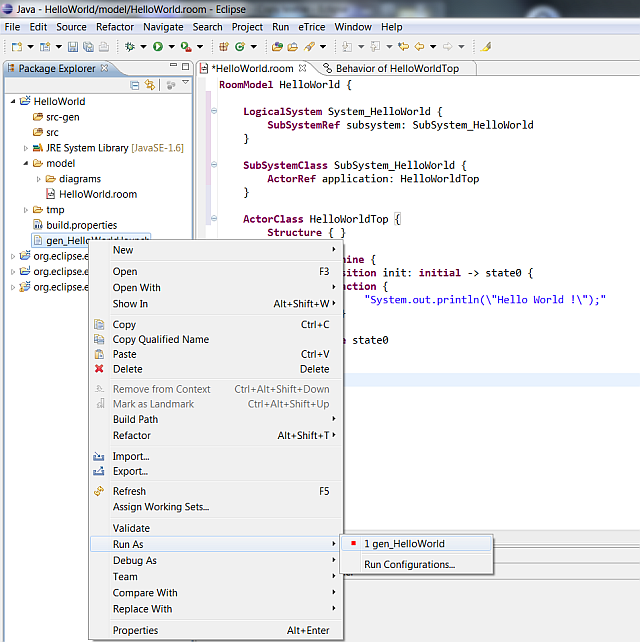
\includegraphics[width=0.8\textwidth]{images/015-HelloWorld06.png}

The source code for the model will be generated into the folder \emph{src-gen}. The main function will be contained in \emph{HelloWorld/Nod\_nodeRef1\_subSysRef1Runner.java}.
Select this file and run it as Java application or use the generated launch configuration \emph{run\_HelloWorld.launch}.

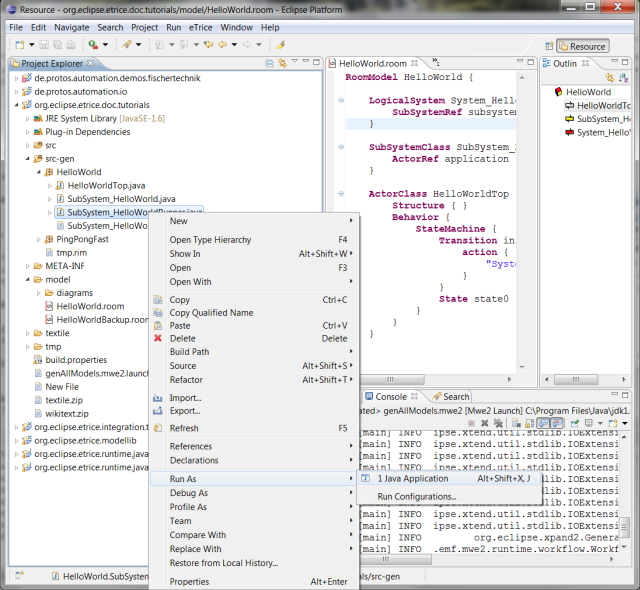
\includegraphics{images/015-HelloWorld07.png}


The Hello World application starts and the string \emph{"Hello World"} will be printed into the console window. To terminate the application the user must enter \emph{quit} in the console window.

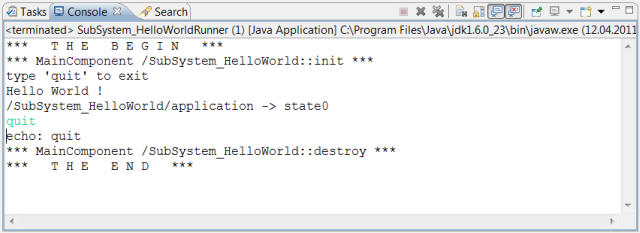
\includegraphics[width=0.6\textwidth]{images/015-HelloWorld08.png}

\subsection{Open the Message Sequence Chart}

For debugging and learning purposes, the application produced a Message Sequence Chart and wrote it to a file. Open the file \emph{subSysRef1\_Async.seq} or \emph{msc.seq} in the folder \emph{HelloWorld/tmp/log/} using the tool Trace2UML. Create the path if not already there.

Trace2UML is an open source MSC viewer and can be obtained here:
\begin{itemize}
\item \href{http://trace2uml.tigris.org/}{Trace2UML project home and download of windows version} 
\item \href{http://apt.astade.de/}{download of the Linux package of the Astade UML tool which contains Trace2UML}
\end{itemize}
After opening the file, you should see something like this:

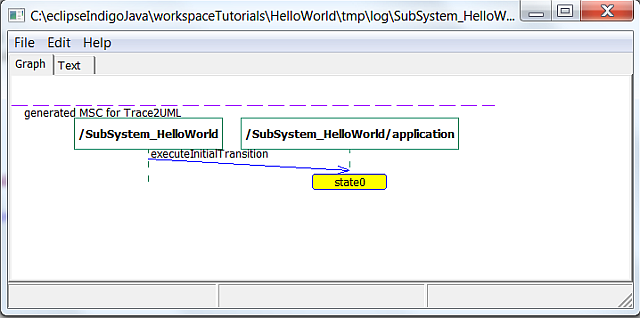
\includegraphics[width=0.6\textwidth]{images/015-HelloWorld09.png}
% !images/015-HelloWorld09.png!

The Actor with the instance path \emph{/LogSys1/subSysRef1/actorRef1} is in the state \emph{state0}. 
This is the simplest possible MSC. The MSCs for further tutorials will contain more information.


\subsection{Summary}

Now you have generated your first \eTrice{} model from scratch. You can switch between diagram editor and 
textual model representation (.room file) and you can see what will be generated during editing and saving the diagram files. 
You should take a look at the generated source files to understand how the state machine is generated and 
the life cycle of the application works. The next tutorials will deal with more complex hierarchies in structure and behavior.

\section{HelloWorld for C}

\subsection{Scope}

In this tutorial you will learn how to create a model for C from scratch. There are some more steps to do 
in C compared to Java. The goal is to get familiar with the additional steps. The Java tutorial is a 
prerequisite for the following explanations. 
You will perform the following steps:

\begin{enumerate}
\item create a new model from scratch for C
\item create structure and behavior similar to Java
\item create a launch configuration for the C code generator
\item setup the C environment
\item generate the source code
\item run the model
\end{enumerate}

Make sure that you have set up the workspace as described in \textit{Setting up the Workspace for C 
Projects}.


\subsection{Create a new model from scratch}

Before you can create a new C-model, you have to create a new C project as described in \textit{Setting up 
the Workspace for C Projects}.
Remember:
\begin{itemize}
\item select the \textit{C/C++} perspective
\item From the main menue select \textit{File->New->C Project}
\item Name the project \textit{HelloWorldC}
\item Project type is \textit{Executable / Empty C Project}
\item Toolchain is \textit{MinGW}
\end{itemize}

The workspace should look like this:

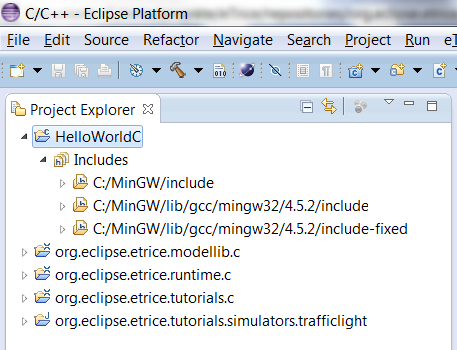
\includegraphics{images/016-HelloWorldC01.png}
% !images/016-HelloWorldC01.png!

The next step is to add the model folder:
Right click on the new project. Select \textit{New->Folder} and name it \textit{model}.

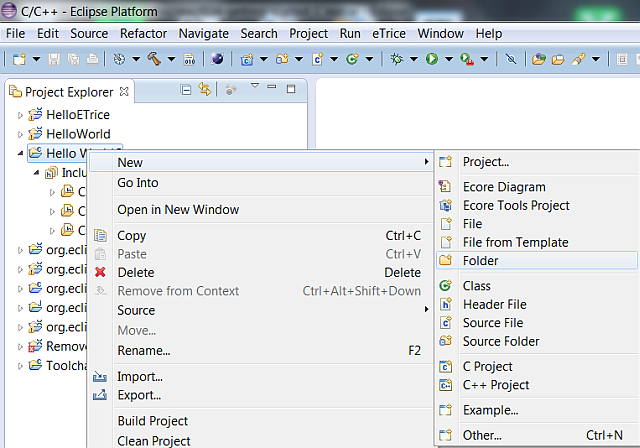
\includegraphics{images/016-HelloWorldC02.png}
% !images/016-HelloWorldC02.png!

Add the model file to the folder. Right click on the new folder. Select \textit{New->file} and name it 
\textit{HelloWorldC.room}.

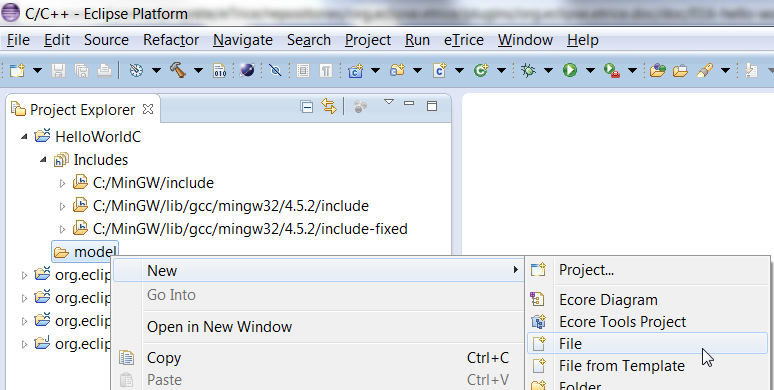
\includegraphics{images/016-HelloWorldC03.png}
% !images/016-HelloWorldC03.png!

Due to the file ending \textit{.room}, the tool will ask you to add the Xtext nature. Answer with 
\textit{Yes}. 

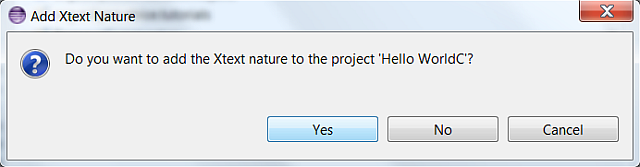
\includegraphics{images/016-HelloWorldC04.png}
% !images/016-HelloWorldC04.png!

The workspace should look like this:

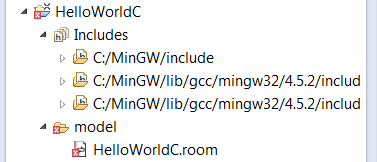
\includegraphics{images/016-HelloWorldC05.png}
% !images/016-HelloWorldC05.png!



\subsection{Create the HelloWorld model}

Once the model file is created and the Xtext nature is added, you can create the model as you did it for 
Java.
Creating the model is not the focus of this tutorial. Therefore copy and paste the following code into 
your model file. Optionally you can open and layout the diagrams.  
Recognize the C specific parts:
\begin{itemize}
\item The action code contains C instead of Java. Later versions will contain a common action language, 
but for the moment the action language is target specific.
\item The application must be shutdown on model level (see also \textit{etRuntimeConfig.h}).  
\end{itemize}

\begin{verbatim} 
RoomModel HelloWorldCModel {
	import room.basic.types.* from "../../org.eclipse.etrice.modellib.c/model/Types.room"
	SubSystemClass HelloWorldCSubSysClass {
		ActorRef HelloETriceTopRef:AHelloWorldCTop 
	}
	ActorClass AHelloWorldCTop {
		Structure { }
		Behavior {
			StateMachine {
				Transition init: initial -> state0 { }
				State state0 {
					entry {
						"printf(\"HelloWorldC !\\n\");"
						"SubSysClass_shutdown();"
						"\t\t\t\t\t\t"
					}
				}
			}
		}
	}	
}
\end{verbatim}

\subsection{Create a launch configuration to start the C code generator}

Other than in Java a launch configuration for the C code generator must be created.

From the \textit{Run} menu select \textit{Run Configurations}

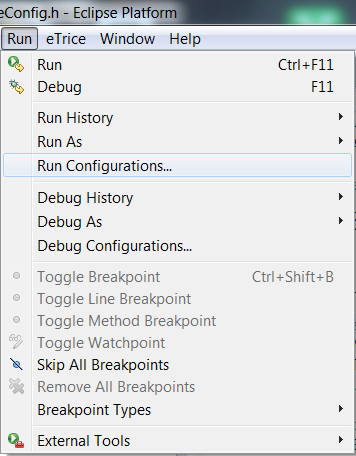
\includegraphics{images/016-HelloWorldC06.png}
% !images/016-HelloWorldC06.png!

Within the dialog select \textit{\eTrice{} C Generator} and click the \textit{New} button to create a new 
launch configuration.

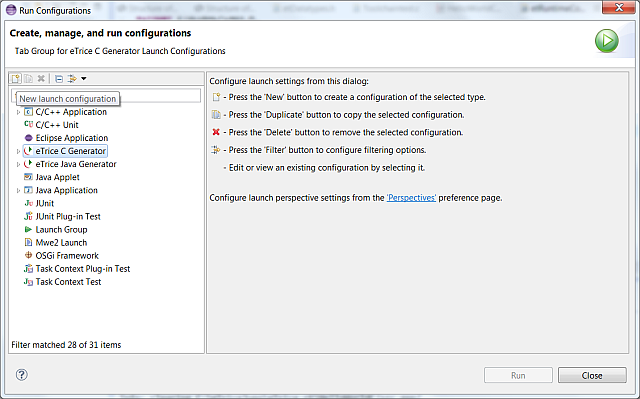
\includegraphics{images/016-HelloWorldC07.png}
% !images/016-HelloWorldC07.png!

A new configuration should be created. Name it \textit{gen\_HelloWorldC} and add the model via one of the 
\textit{add} buttons.

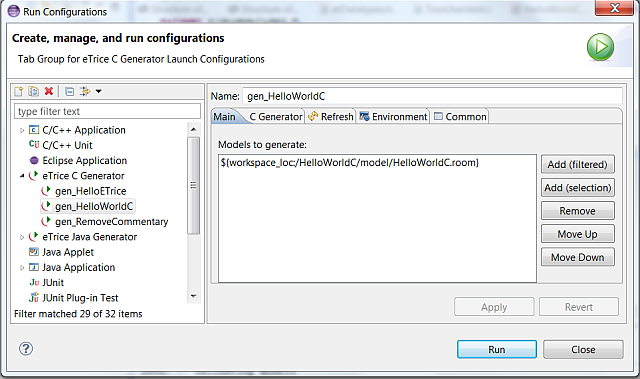
\includegraphics{images/016-HelloWorldC08.png}
% !images/016-HelloWorldC08.png!

In the \textit{Refresh} tab select \textit{The entire workspace} 

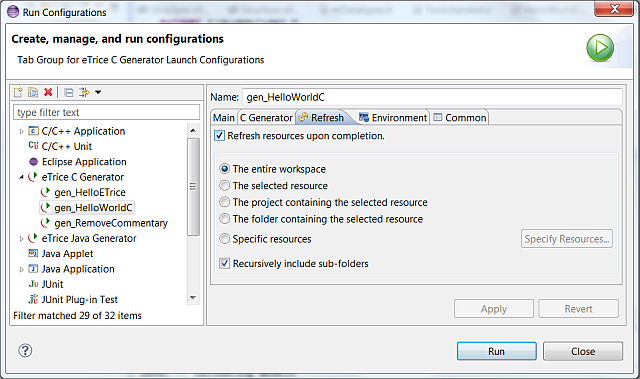
\includegraphics{images/016-HelloWorldC09.png}
% !images/016-HelloWorldC09.png!

In the \textit{Common} tab select \textit{Shared file} and add the \textit{HelloWorldC} project via the 
\textit{Browse} button.

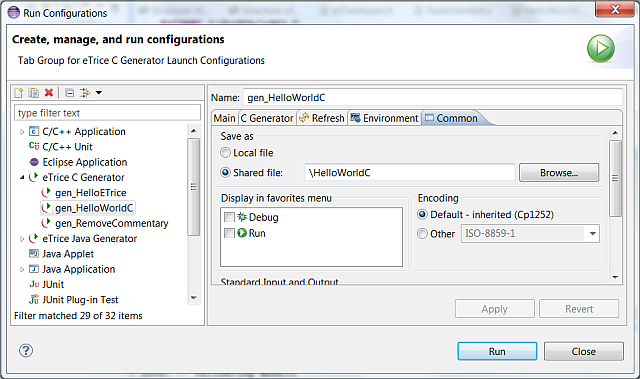
\includegraphics{images/016-HelloWorldC10.png}
% !images/016-HelloWorldC10.png!

Apply your changes. The new configuration should now exist in your workspace.

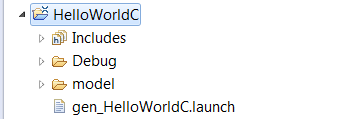
\includegraphics{images/016-HelloWorldC11.png}
% !images/016-HelloWorldC11.png!


\subsection{Generate the code}

Now you can generate the code as you know it from Java. Right click on the launch configuration and run it 
as \textit{gen\_HelloWorldC}.

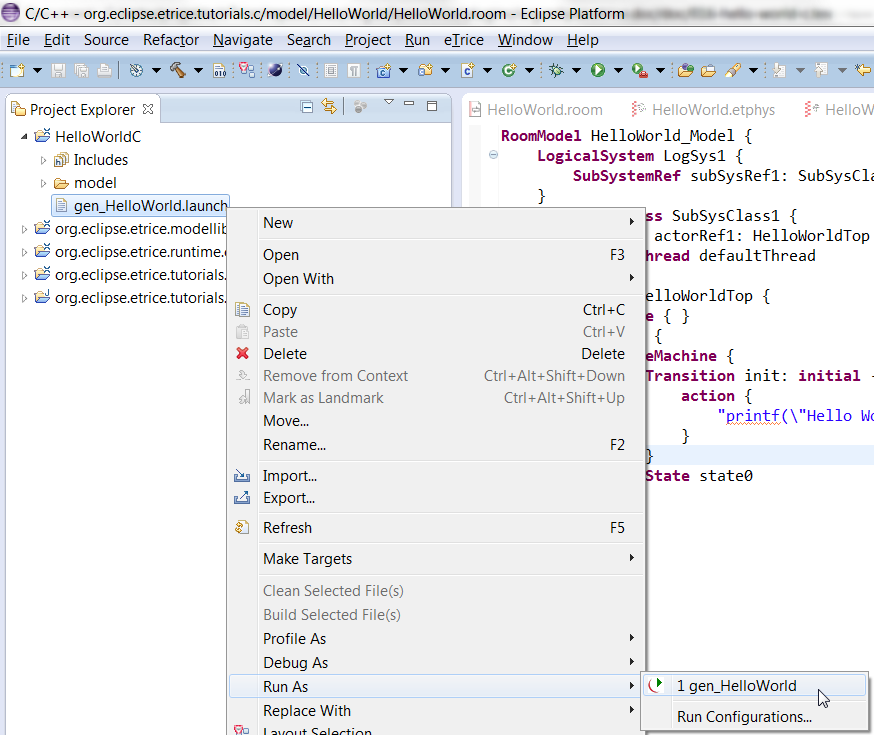
\includegraphics{images/016-HelloWorldC12.png}
% !images/016-HelloWorldC12.png!

The code should be generated.

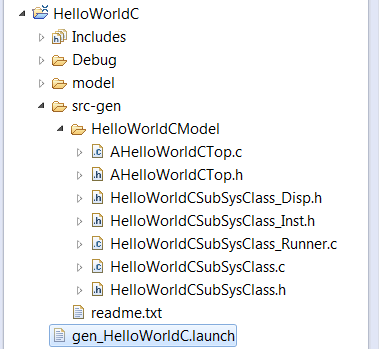
\includegraphics{images/016-HelloWorldC13.png}
% !images/016-HelloWorldC13.png!

\subsection{Setup the include path}

Before you can build the application you must setup the include path for the runtime system. Right click 
the project and select \textit{Properties}. Add the include path as described in \textit{setting up the 
workspace}.

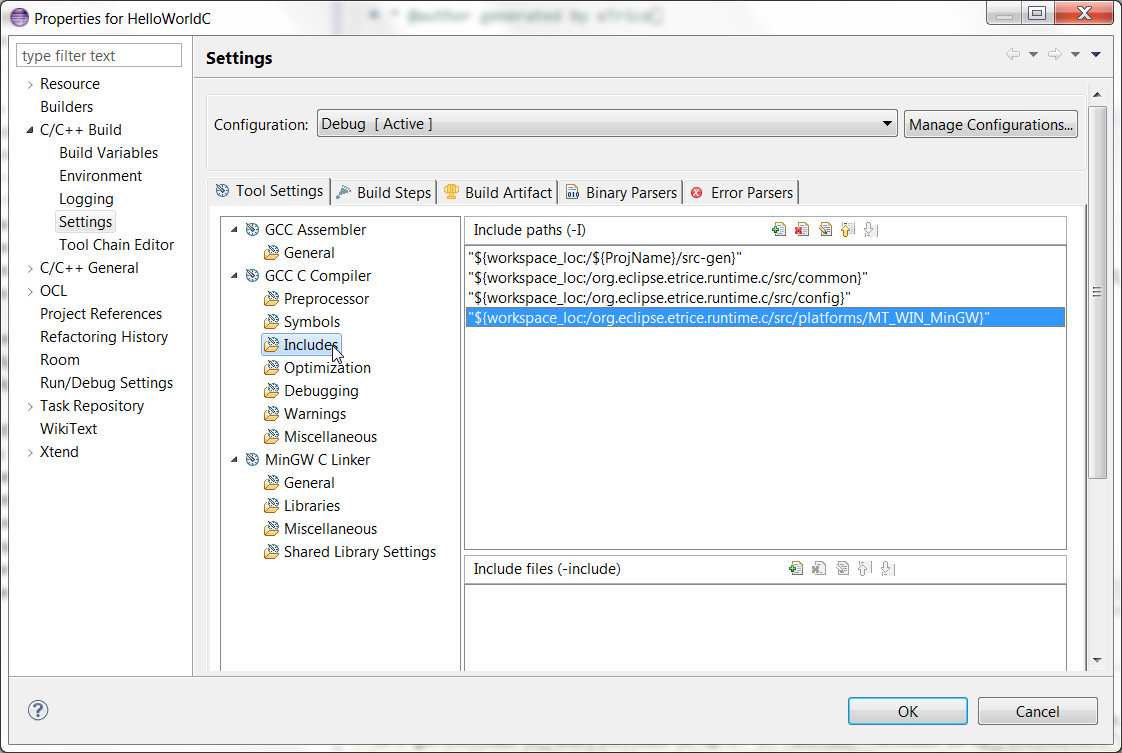
\includegraphics{images/016-HelloWorldC14.png}
% !images/016-HelloWorldC14.png!

Add the runtime library.

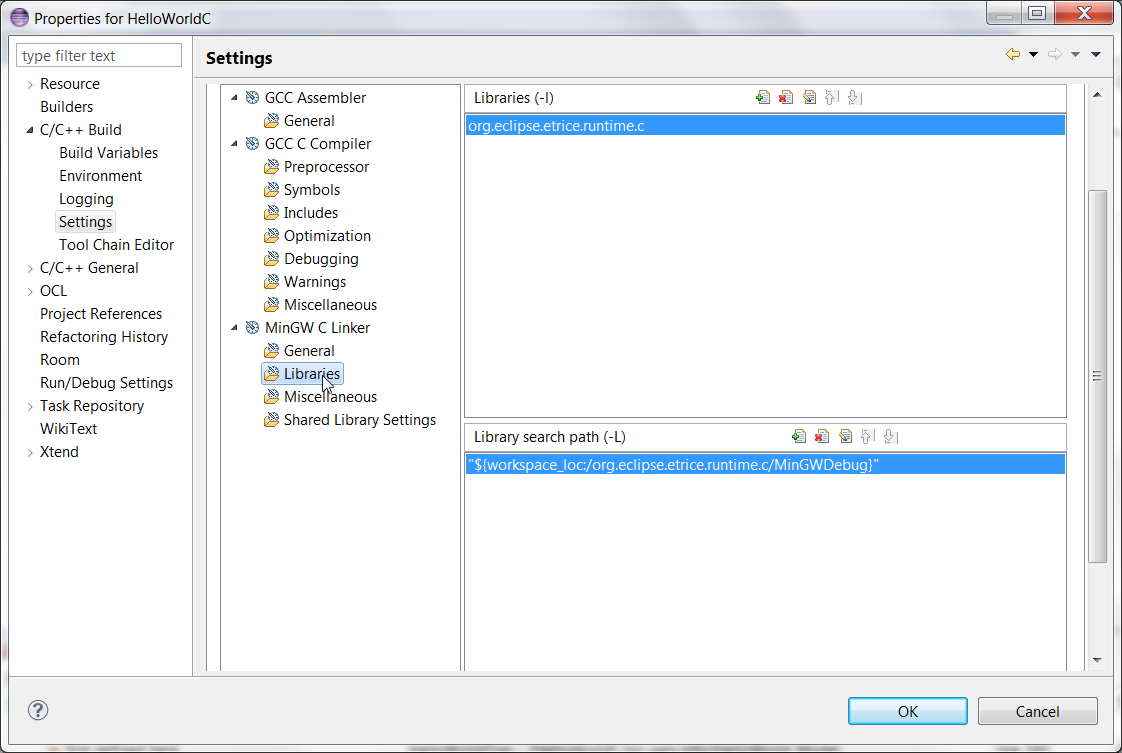
\includegraphics{images/016-HelloWorldC15.png}
% !images/016-HelloWorldC15!

Recognize the name of the library ("org.eclipse.etrice.runtime.c"). The library file on your disk is 
"liborg.eclipse.etrice.runtime.c.a". 

\subsection{Build and run the model}

Now you can build the application. Click the build button to build the application.
Run the application as \textit{Local C/C++ Application}.
Verify the output.

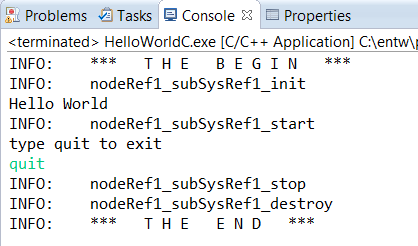
\includegraphics{images/016-HelloWorldC16.png}
% !images/016-HelloWorldC16.png!

\subsection{Summary}

You are now familiar with all necessary steps to create, build and run an \eTrice{} C model from scratch. You 
are able to create a launch configuration to start the code generator and to perform all necessary 
settings to compile and link the application.  

The next tutorial provides an exercise to get more familiar with these working steps.

%\chapter{Tutorial Blinky (Java)}

\section{Scope}

This tutorial describes how to use the \textit{TimingService}, how to combine a generated model with manual code and how to model a hierarchical state machine. The idea of the tutorial is to switch a LED on and off. The behavior of the LED should be: blinking in a one second interval for 5 seconds, stop blinking for 5 seconds, blinking, stop,...  
For this exercise we will use a little GUI class that will be used in more sophisticated tutorials too. The GUI simulates a pedestrian traffic crossing. For now, just a simple LED simulation will be used from the GUI. 

After the exercise is created you must copy the GUI to your src directory (see below).

The package contains four java classes which implements a small window with a 3-light traffic light which simulates the signals for the car traffic and a 2-light traffic light which simulates the pedestrian signals.

The GUI looks like this:

\includegraphics{images/020-Blinky08.png}
% !images/020-Blinky08.png!

Within this tutorial we will just toggle the yellow light.

You will perform the following steps:

\begin{enumerate}
\item create a new model from scratch
\item define a protocol
\item create an actor structure
\item create a hierarchical state machine
\item use the predefined \textit{TimingService}
\item combine manual code with generated code
\item build and run the model
\item open the message sequence chart
\end{enumerate}

\section{Create a new model from scratch}

Remember the exercise \textit{HelloWorld}.
Create a new eTrice project and name it \textit{Blinky}.

To use the GUI please copy the package \textit{org.eclipse.etrice.tutorials.PedLightGUI} from \textit{org.eclipse.etrice.tutorials/src} to your *src* directory \textit{Blinky/src}. For this tutorial you must remove the error markers by editing the file \textit{PedestrianLightWndNoTcp.java}. Appropriate comments are provided to remove the error markers for this turorial.

Open the \textit{Blinky.room} file and copy the following code into the file or use content assist to create the model.

\begin{verbatim} 
RoomModel Blinky {

    LogicalSystem System_Blinky {
        SubSystemRef subsystem : SubSystem_Blinky
    }

    SubSystemClass SubSystem_Blinky {
        ActorRef application : BlinkyTop
    }

    ActorClass BlinkyTop {
    }
}
\end{verbatim}

\section{Add two additional actor classes}

Position the cursor outside any class definition and right click the mouse within the editor window. From the context menu select \textit{Content Assist}  

\includegraphics[width=0.8\textwidth]{images/020-Blinky02.png}
% !images/020-Blinky02.png!

Select \textit{ActorClass - actor class skeleton} and name it \textit{Blinky}.

\includegraphics[width=0.8\textwidth]{images/020-Blinky01.png}
% !images/020-Blinky01.png! 

Repeat the described procedure and name the new actor \textit{BlinkyController}.

With Ctrl+Shift+F you can beautify the model code. 

Save the model and visit the outline view.

\section{Create a new protocol}

With the help of \textit{Content Assist} create a \textit{ProtocolClass} and name it \textit{BlinkyControlProtocol}.
Inside the brackets use the \textit{Content Assist} (CTRL+Space) to create two incoming messages called \textit{start} and \textit{stop}.

The resulting code should look like this:

\includegraphics[width=0.8\textwidth]{images/020-Blinky03.png}
% !images/020-Blinky03.png!

With Ctrl-Shift+F or selecting \textit{Format} from the context menu you can format the text. Note that all elements are displayed in the outline view.

\section{Import the Timing Service}

Switching on and off the LED is timing controlled. The timing service is provided from the model library and must be imported before it can be used from the model.

This is the first time you use an element from the modellib. Make sure that your Java Build Path has the appropriate entry to the modellib. Otherwise the jave code, which will be generated from the modellib, can not be referenced.
(right click to \textit{Blinky} and select properties. Select the \textit{Java Build Path} tab) 
  
\includegraphics[width=0.8\textwidth]{images/020-Blinky16.png}
% !images/020-Blinky16.png! 

After the build path is set up return to the model and navigate the cursor at the beginning of the model and import the timing service: 

\begin{small}
\begin{verbatim}
RoomModel Blinky {
    
    import room.basic.service.timing.* from 
		"../../org.eclipse.etrice.modellib/models/TimingService.room" 
    
    LogicalSystem System_Blinky {
        SubSystemRef subsystem: SubSystem\_Blinky
    }
}
...     
\end{verbatim}
\end{small}

Make sure that the path fits to your folder structure. The original tutorial code is different due to the folder structure.  

Now it can be used within the model. Right click to \textbf{SubSystem\_Blinky} within the outline view. Select \textit{Edit Structure}. The \textit{application} is already referenced in the subsystem. Drag and Drop an \textit{ActorRef} to the \textbf{SubSystem\_Blinky} and name it \textit{timingService}. From the actor class drop down list select \textit{room.basic.service.timing.ATimingService}. Draw a \textit{LayerConnection} from \textit{application} to each service provision point (SPP) of the \textit{timingService}. The resulting structure should look like this:

\includegraphics[width=0.8\textwidth]{images/020-Blinky06.png}
% !images/020-Blinky06.png! 

The current version of eTrice does not provide a graphical element for a service access point (SAP). Therefore the SAPs to access the timing service must be added in the .room file. Open the \textit{Blinky.room} file and navigate to the \textit{Blinky} actor. Add the following line to the structure of the actor:

\begin{verbatim}SAP timer: room.basic.service.timing.PTimeout \end{verbatim}

Do the same thing for \textit{BlinkyController}.

The resulting code should look like this:

\includegraphics[width=0.8\textwidth]{images/020-Blinky07.png}
% !images/020-Blinky07.png!


\section{Finish the model structure}

From the outline view right click to \textit{Blinky} and select \textit{Edit Structure}. Drag and Drop an \textit{Interface Port} to the boarder of the \textit{Blinky} actor. Note that an interface port is not possible inside the actor. Name the port \textit{ControlPort} and select \textit{BlinkyControlProtocol} from the drop down list. Uncheck \textit{Conjugated} and \textit{Is Relay Port}. Click \textit{ok}. The resulting structure should look like this:

\includegraphics[width=0.8\textwidth]{images/020-Blinky04.png}
% !images/020-Blinky04.png!

Repeat the above steps for the \textit{BlinkyController}. Make the port \textit{Conjugated}

Keep in mind that the protocol defines \textit{start} and \textit{stop} as incoming messages. \textit{Blinky} receives this messages and therefore \textit{Blinky}'s \textit{ControlPort} must be a regular port and \textit{BlinkyController}'s \textit{ControlPort} must be a conjugated port.


From the outline view right click \textit{BlinkyTop} and select \textit{Edit Structure}.

Drag and Drop an \textit{ActorRef} inside the \textit{BlinkyTop} actor. Name it \textit{blinky}. From the actor class drop down list select \textit{Blinky}. Do the same for \textit{controller}. Connect the ports via the binding tool. The resulting structure should look like this:

\includegraphics[width=0.8\textwidth]{images/020-Blinky05.png}
% !images/020-Blinky05.png!

\section{Implement the Behavior}

The application should switch on and off the LED for 5 seconds in a 1 second interval, then stop blinking for 5 seconds and start again. To implement this behavior we will implement two FSMs. One for the 1 second interval and one for the 5 second interval. The 1 second blinking should be implemented in \textit{Blinky}. The 5 second interval should be implemented in \textit{BlinkyController}. First implement the Controller.

Right click to \textit{BlinkyController} and select \textit{Edit Behavior}.
Drag and Drop the \textit{Initial Point} and two \textit{States} into the top state. Name the states \textit{on} and \textit{off}. 
Use the \textit{Transition} tool to draw transitions from \textit{init} to \textit{on} from \textit{on} to \textit{off} and from \textit{off} to \textit{on}.

Open the transition dialog by double click the arrow to specify the trigger event and the action code of each transition. Note that the initial transition does not have a trigger event.

The transition dialog should look like this:

\includegraphics[width=0.8\textwidth]{images/020-Blinky09.png}
% !{width=500px}images/020-Blinky09.png! 

The defined ports will be generated as a member attribute of the actor class from type of the attached protocol. So, to send e message you must state \textit{port.message(param);}. In this example \textit{ControlPort.start()} sends the \textit{start} message via the \textit{ControlPort} to the outside world. Assuming that \textit{Blinky} is connected to this port, the message will start the one second blinking FSM. It is the same thing with the \textit{timer}. The SAP is also a port and follows the same rules. So it is clear that \textit{timer.Start(5000);} will send the \textit{Start} message to the timing service. The timing service will send a \textit{timeoutTick} message back after 5000ms.

Within each transition the timer will be restarted and the appropriate message will be sent via the \textit{ControlPort}. 

The resulting state machine should look like this:
(Note that the arrows peak changes if the transition contains action code.)

\includegraphics[width=0.8\textwidth]{images/020-Blinky10.png}
% !images/020-Blinky10.png!

Save the diagram and inspect the \textit{Blinky.room} file. The \textit{BlinkyController} should look like this:

\includegraphics[width=0.8\textwidth]{images/020-Blinky11.png}
% !images/020-Blinky11.png! 
 
Now we will implement \textit{Blinky}. Due to the fact that \textit{Blinky} interacts with the GUI class a view things must to be done in the model file.

Double click \textit{Blinky} in the outline view to navigate to \textit{Blinky} within the model file.
Add the following code:
(type it or simply copy it from the tutorial project)

\includegraphics[width=0.8\textwidth]{images/020-Blinky12.png}
% !images/020-Blinky12.png! 

\textit{usercode1} will be generated at the beginning of the file, outside the class definition. \textit{usercode2} will be generated within the class definition. The code imports the GUI class and instantiates the window class. Attributes for the carLights and pedLights will be declared to easily access the lights in the state machine.
The Operation \textit{destroyUser()} is a predefined operation that will be called during shutdown of the application. Within this operation, cleanup of manual coded classes can be done.
 
Now design the FSM of \textit{Blinky}. Remember, as the name suggested \textit{blinking} is a state in which the LED must be switched on and off. We will realize that by an hierarchical FSM in which the \textit{blinking} state has two sub states.

Open the behavior diagram of \textit{Blinky} by right clicking the \textit{Blinky} actor in the outline view. Create two states named \textit{blinking} and \textit{off}. Right click to \textit{blinking} and create a subgraph.

\includegraphics[width=0.8\textwidth]{images/020-Blinky13.png}
% !images/020-Blinky13.png!

Create the following state machine. The trigger events between \textit{on} and \textit{off} are the \textit{timeoutTick} from the \textit{timer} port. 

\includegraphics[width=0.8\textwidth]{images/020-Blinky14.png}
% !images/020-Blinky14.png!

Create entry code for both states by right clicking the state and select \textit{Edit State...}

Entry code of \textit{on} is:

\begin{verbatim}
timer.Start(1000);
carLights.setState(TrafficLight3.YELLOW); 
\end{verbatim}

 
Entry code  of \textit{off} is:

\begin{verbatim}
timer.Start(1000);
carLights.setState(TrafficLight3.OFF);
\end{verbatim}

Navigate to the Top level state by double clicking the \textit{/blinking} state. Create the following state machine:

\includegraphics[width=0.8\textwidth]{images/020-Blinky15.png}
% !images/020-Blinky15.png!

The trigger event from \textit{off} to \textit{blinking} is the \textit{start} event from the \textit{ControlPort}.The trigger event from \textit{blinking} to \textit{off} is the \textit{stop} event from the \textit{ControlPort}.
Note: The transition from \textit{blinking} to \textit{off} is a so called group transition. This is a outgoing transition from a super state (state with sub states) without specifying the concrete leave state (state without sub states). An incoming transition to a super state is called history transition.   

Action code of the init transition is:

\begin{verbatim}
carLights = light.getCarLights();
pedLights = light.getPedLights();
carLights.setState(TrafficLight3.OFF);
pedLights.setState(TrafficLight2.OFF);
\end{verbatim}

Action code from \textit{blinking} to \textit{off} is:

\begin{verbatim}
timer.Kill();
carLights.setState(TrafficLight3.OFF); 
\end{verbatim}

The model is complete now. You can run and debug the model as described in getting started. Have fun.

The complete model can be found in /org.eclipse.etrice.tutorials/model/Blinky.

\section{Summary}

Run the model and take a look at the generated MSCs. Inspect the generated code to understand the runtime model of eTrice. Within this tutorial you have learned how to create a hierarchical FSM with group transitions and history transitions and you have used entry code. You are now familiar with the basic features of eTrice. The further tutorials will take this knowledge as a precondition.

%\chapter{Tutorial Sending Data (Java)}

\section{Scope}

This tutorial shows how data will be sent in a eTrice model. Within the example you will create two actors (MrPing and MrPong). MrPong will simply loop back every data it received.
MrPing will send data and verify the result.   

You will perform the following steps:

\begin{enumerate}
\item create a new model from scratch
\item create a data class
\item define a protocol with attached data
\item create an actor structure
\item create two simple state machines
\item build and run the model
\end{enumerate}

\section{Create a new model from scratch}

Remember exercise \textit{HelloWorld}.
Create a new eTrice project and name it \textit{SendingData}.
Open the \textit{SendingData.room} file and copy the following code into the file or use content assist to create the model.


\begin{verbatim} 
RoomModel SendingData {
    LogicalSystem SendingData_LogSystem {
        SubSystemRef SendingDataAppl:SendingData_SubSystem 
    }
    SubSystemClass SendingData_SubSystem {
        ActorRef SendigDataTopRef:SendingDataTop 
    }
    ActorClass SendingDataTop {
    }
}
\end{verbatim}

\section{Add a data class}

Position the cursor outside any class definition and right click the mouse within the editor window. From the context menu select \textit{Content Assist} (or Ctrl+Space).  

\includegraphics{images/025-SendingData01.png}
% !images/025-SendingData01.png!

Select \textit{DataClass - data class skeleton} and name it \textit{DemoData}.
Remove the operations and add the following Attributes:

\begin{verbatim}
DataClass DemoData {
    Attribute int32Val: int32 = "4711"
    Attribute int8Array [ 10 ]: int8 = "{1,2,3,4,5,6,7,8,9,10}"
    Attribute float64Val: float64 = "0.0"
    Attribute stringVal: string = "\"empty\""
}
\end{verbatim}

Save the model and visit the outline view.
Note that the outline view contains all data elements as defined in the model. 

\section{Create a new protocol}

With the help of \textit{Content Assist} create a \textit{ProtocolClass} and name it \textit{PingPongProtocol}. Create the following messages:

\begin{verbatim} 
ProtocolClass PingPongProtocol {
    incoming {
        Message ping(data: DemoData)
        Message pingSimple(data:int32)
    }
    outgoing {
        Message pong(data: DemoData)
        Message pongSimple(data:int32)
    }
}    
\end{verbatim}

\section{Create MrPing and MrPong Actors}

With the help of \textit{Content Assist} create two new actor classes and name them \textit{MrPing} and \textit{MrPong}. The resulting model should look like this:

\begin{verbatim}
RoomModel SendingData {

    LogicalSystem SendingData_LogSystem {
        SubSystemRef SendingDataAppl: SendingData_SubSystem
    }

    SubSystemClass SendingData_SubSystem {
        ActorRef SendigDataTopRef: SendingDataTop
    }

    ActorClass SendingDataTop { }

    DataClass DemoData {
        Attribute int32Val: int32 = "4711"
        Attribute int8Array [ 10 ]: int8 = "{1,2,3,4,5,6,7,8,9,10}"
        Attribute float64Val: float64 = "0.0"
        Attribute stringVal: string = "\"empty\""
    }

    ProtocolClass PingPongProtocol {
        incoming {
            Message ping(data: DemoData)
            Message pingSimple(data: int32)
        }
        outgoing {
            Message pong(data: DemoData)
            Message pongSimple(data: int32)
        }
    }

    ActorClass MrPing {
        Interface { }
        Structure { }
        Behavior { }
    }

    ActorClass MrPong {
        Interface { }
        Structure { }
        Behavior { }
    }
} 

\end{verbatim}

The outline view should look like this:

\includegraphics{images/025-SendingData03.png}
% !images/025-SendingData03.png!

\section{Define Actor Structure and Behavior}

Save the model and visit the outline view. Within the outline view, right click on the \textit{MrPong} actor and select \textit{Edit Structure}. Select an \textit{Interface Port} from the toolbox and add it to MrPong. Name the Port \textit{PingPongPort} and select the \textit{PingPongProtocol}.

\includegraphics{images/025-SendingData02.png}
% !images/025-SendingData02.png!

Do the same with MrPing but mark the port as \textit{conjugated}

\subsection{Define MrPongs behavior}

Within the outline view, right click MrPong and select \textit{Edit Behavior}. Create the following state machine:

\includegraphics{images/025-SendingData04.png}
% !images/025-SendingData04.png!

The transition dialogues should look like this:
For \textit{ping}:

\includegraphics{images/025-SendingData05.png}
% !images/025-SendingData05.png!

For \textit{pingSimple}:

\includegraphics{images/025-SendingData06.png}
% !images/025-SendingData06.png!


\subsection{Define MrPing behavior}

Within the outline view double click MrPing. Navigate the cursor to the behavior of MrPing. With the help of content assist create a new operation.

\includegraphics{images/025-SendingData07.png}
% !images/025-SendingData07.png!

Name the operation \textit{printData} and define the DemoData as a parameter.

Fill in the following code:

\begin{verbatim}
Operation printData(d: DemoData) : void {
            "System.out.printf(\"d.int32Val: %d\\n\",d.int32Val);"
            "System.out.printf(\"d.float64Val: %f\\n\",d.float64Val);"
            "System.out.printf(\"d.int8Array: \");"
            "for(int i = 0; i<d.int8Array.length; i++) {"
            "System.out.printf(\"%d \",d.int8Array[i]);}"
            "System.out.printf(\"\\nd.stringVal: %s\\n\",d.stringVal);"
}
\end{verbatim}

For MrPing create the following state machine:
(Remember that you can copy and paste the action code from the tutorial directory.)

\includegraphics{images/025-SendingData08.png}
% !images/025-SendingData08.png!

The transition dialogues should look like this:

For \textit{init}:

\includegraphics{images/025-SendingData09.png}
% !images/025-SendingData09.png!

For \textit{wait1}:

\includegraphics{images/025-SendingData10.png}
% !images/025-SendingData10.png!

For \textit{next}:

\includegraphics{images/025-SendingData11.png}
% !images/025-SendingData11.png!

For \textit{wait2}:

\includegraphics{images/025-SendingData12.png}
% !images/025-SendingData12.png!

\section{Define the top level}

Open the Structure from SendingDataTop and add MrPing and MrPong as a reference. Connect the ports.

\includegraphics{images/025-SendingData13.png}
% !images/025-SendingData13.png!

The model is finished now and can be found in /org.eclipse.etrice.tutorials/model/SendingData.

\section{Generate and run the model}

Generate the code by right click to \textbf{gen\_SendingData.launch} and run it as \textbf{gen\_SendingData}. Run the model. 
The output should look like this:

\begin{verbatim}
type 'quit' to exit
/SendingData_SubSystem/SendigDataTopRef/ref0 -> waitForPongSimple
/SendingData_SubSystem/SendigDataTopRef/ref1 -> looping
/SendingData_SubSystem/SendigDataTopRef/ref1 -> looping
data: 1
/SendingData_SubSystem/SendigDataTopRef/ref0 -> waitForPongSimple
/SendingData_SubSystem/SendigDataTopRef/ref1 -> looping
data: 2
/SendingData_SubSystem/SendigDataTopRef/ref0 -> waitForPongSimple
/SendingData_SubSystem/SendigDataTopRef/ref1 -> looping
data: 3
/SendingData_SubSystem/SendigDataTopRef/ref0 -> waitForPongSimple
/SendingData_SubSystem/SendigDataTopRef/ref1 -> looping
data: 4
/SendingData_SubSystem/SendigDataTopRef/ref0 -> waitForPongSimple
/SendingData_SubSystem/SendigDataTopRef/ref1 -> looping
data: 5
/SendingData_SubSystem/SendigDataTopRef/ref0 -> waitForPongSimple
/SendingData_SubSystem/SendigDataTopRef/ref1 -> looping
data: 6
/SendingData_SubSystem/SendigDataTopRef/ref0 -> waitForPongSimple
/SendingData_SubSystem/SendigDataTopRef/ref1 -> looping
data: 7
/SendingData_SubSystem/SendigDataTopRef/ref0 -> waitForPongSimple
/SendingData_SubSystem/SendigDataTopRef/ref1 -> looping
data: 8
/SendingData_SubSystem/SendigDataTopRef/ref0 -> waitForPongSimple
/SendingData_SubSystem/SendigDataTopRef/ref1 -> looping
data: 9
/SendingData_SubSystem/SendigDataTopRef/ref0 -> waitForPongSimple
/SendingData_SubSystem/SendigDataTopRef/ref1 -> looping
data: 10
/SendingData_SubSystem/SendigDataTopRef/ref0 -> waitForPong
/SendingData_SubSystem/SendigDataTopRef/ref1 -> looping
/SendingData_SubSystem/SendigDataTopRef/ref1 -> looping
d.int32Val: 4711
d.float64Val: 0,000000
d.int8Array: 1 2 3 4 5 6 7 8 9 10 
d.stringVal: empty
/SendingData_SubSystem/SendigDataTopRef/ref0 -> waitForPong
d.int32Val: 815
d.float64Val: 3,141234
d.int8Array: 100 101 102 103 104 105 106 107 108 109 
d.stringVal: some contents
/SendingData_SubSystem/SendigDataTopRef/ref0 -> waitForPong
quit
echo: quit
\end{verbatim}

\section{Summary}

Within the first loop an integer value will be incremented by \textit{MrPong} and sent back to \textit{MrPing}. As long as the guard is true \textit{MrPing} sends back the value.

Within the \textit{next} transition, \textit{MrPing} creates a data class and sends the default values. Then \textit{MrPing} changes the values and sends the class again. At this point you should note that during the send operation, a copy of the data class will be created and sent. Otherwise it would not be possible to send the same object two times, even more it would not be possible to send a stack object at all. This type of data passing is called \textit{sending data by value}.
However, for performance reasons some applications requires \textit{sending data by reference}. In this case the user is responsible for the life cycle of the object. In Java the VM takes care of the life cycle of an object. This is not the case for C/C++. Consider that a object which is created within a transition of a state machine will be destroyed when the transition is finished. The receiving FSM would receive an invalid reference. Therefore care must be taken when sending references.      

For sending data by reference you simply have to add the keyword \textit{ref} to the protocol definition.
 
\begin{verbatim}Message ping(data: DemoData ref)\end{verbatim}

Make the test and inspect the console output.

%\chapter{Tutorial Pedestrian Lights (Java)}

\section{Scope}

The scope of this tutorial is to demonstrate how to receive model messages from outside the model. Calling methods which are not part of the model is simple and you have already done this within the blinky tutorial (this is the other way round: model => external code). Receiving events from outside the model is a very common problem and a very frequently asked question. Therefore this tutorial shows how an external event (outside the model) can be received by the model.

This tutorial is not like hello world or blinky. Being familiar with the basic tool features is mandatory for this tutorial. The goal is to understand the mechanism not to learn the tool features.

The idea behind the exercise is, to control a Pedestrian crossing light. We will use the same GUI as for the blinky tutorial but now we will use the \textit{REQUEST} button to start a FSM, which controls the traffic lights.

\includegraphics{images/020-Blinky08}
% !images/020-Blinky08.png!

The \textit{REQUEST} must lead to a model message which starts the activity of the lights.

There are several possibilities to receive external events (e.g. TCP/UDP Socket, using OS messaging mechanism), but the easiest way is, to make a port usable from outside the model. To do that a few steps are necessary:
\begin{enumerate}
\item specify the messages (within a protocol) which should be sent into the model
\item model an actor with a port (which uses the specified protocol) and connect the port to the receiver 
\item the external code should know the port (import of the port class)
\item the external code should provide a registration method, so that the actor is able to allow access to this port
\item the port can be used from the external code
\end{enumerate}

\section{Setup the model}

\begin{itemize}
\item Use the \textit{New Model Wizzard} to create a new eTrice project and name it \textit{PedLightsController}.
\item Copy the package \textit{org.eclipse.etrice.tutorials.PedLightGUI} to your \textit{src} directory (see blinky tutorial).
\item In PedestrianLightWndNoTcp.jav uncomment line 15 (import), 36, 122 (usage) and 132-134 (registration). The error markers will disappear after the code is generated from the model.
\item \begin{flushleft}Copy the model from /org.eclipse.etrice.tutorials/model/PedLightsController to your model file, or run the model directly in the tutorial directory.\end{flushleft} 
\item Adapt the import statement to your path.
\end{itemize}

\begin{small}
\begin{verbatim} 
import room.basic.service.timing.* from 
	"../../org.eclipse.etrice.modellib/models/TimingService.room" 
\end{verbatim}
\end{small}

\begin{itemize}
\item Generate the code from the model.
\item Add the org.eclipse.etrice.modellib to the Java Class Path of your project.
\item All error markers should be disappeared and the model should be operable. 
\item Arrange the Structure and the Statemachines to understand the model
\end{itemize}

\includegraphics[width=\linewidth]{images/030-PedLights01}
% !images/030-PedLights01.png!
The \textit{GuiAdapter} represents the interface to the external code. It registers its \textit{ControlPort} by the external code.

\includegraphics[width=\linewidth]{images/030-PedLights02}
% !images/030-PedLights02.png!
Visit the initial transition to understand the registration. The actor handles the incoming messages as usual and controls the traffic lights as known from blinky. 

\includegraphics[width=\linewidth]{images/030-PedLights03}
% !images/030-PedLights03.png!
The \textit{Controller} receives the \textit{start} message and controls the timing of the lights. Note that the \textit{start} message will be sent from the external code whenever the \textit{REQUEST} button is pressed.

\begin{itemize}
\item  Visit the model and take a closer look to the following elements:
\begin{enumerate}
\item PedControlProtocol => notice that the start message is defined as usual
\item Initial transition of the \textit{GuiAdapter} => see the registration
\item The \textit{Controller} => notice that the \textit{Controller} receives the external message (not the \textit{GuiAdapter}). The \textit{GuiAdapter} just provides its port and handles the incoming messages.
\item Visit the hand written code => see the import statement of the protocol class and the usage of the port.
\end{enumerate}
\item Generate and test the model
\item Take a look at the generated MSC => notice that the start message will shown as if the \textit{GuiAdapter} had sent it.
\end{itemize}

\includegraphics[width=\linewidth]{images/030-PedLights04}
% !images/030-PedLights04.png!

\section{Why does it work and why is it safe?}

The tutorial shows that it is generally possible to use every port from outside the model as long as the port knows its peer. This is guaranteed by describing protocol and the complete structure (especially the bindings) within the model. 
The only remaining question is: Why is it safe and does not violate the \textbf{run to completion} semantic. To answer this question, take a look at the \textit{MessageService.java} from the runtime environment. There you will find the receive method which puts each message into the queue. 

\begin{verbatim}
    @Override
    public synchronized void receive(Message msg) {
        if (msg!=null) {
            messageQueue.push(msg);
            notifyAll(); // wake up thread to compute message
        }
    }
\end{verbatim}

This method is synchronized. That means, regardless who sends the message, the queue is secured. If we later on (e.g. for performance reasons in C/C++) distinguish between internal and external senders (same thread or not), care must be taken to use the external (secure) queue.


\chapter{ROOM Concepts}
\label{sec:room_concepts}

This chapter gives an overview over the ROOM language elements and their textual and graphical notation.
The formal ROOM grammar based on Xtext (EBNF) you can find in the \eTrice{} repository:
\url{http://git.eclipse.org/c/etrice/org.eclipse.etrice.git/plain/plugins/org.eclipse.etrice.core.room/src/org/eclipse/etrice/core/Room.xtext}

\section{Actors}

\subsection{Description}
 
The actor is the basic structural building block for building systems with ROOM. An actor can be refined 
hierarchically and thus can be of arbitrarily large scope. Ports define the interface of an actor.
An actor can also have a behavior usually defined by a finite state machine.

\subsection{Motivation}

\begin{itemize}
\item Actors enable the construction of hierarchical structures by composition and layering
\item Actors have their own logical thread of execution
\item Actors can be freely deployed
\item Actors define potentially re-usable blocks
\end{itemize}

\subsection{Notation}

\lstset{numbers=none, language=ROOM}

\begin{table}
\caption{Actor Class Notation}
\begin{tabular}{|l|l|l|}
\hline
 \textbf{Element} & \textbf{Graphical Notation} & \textbf{Textual Notation} \\ \hline
  ActorClass & 
  \includegraphics[scale=0.7]{images/040-ActorClassNotation.png} & 
  \begin{lstlisting}
ActorClass ActorClass2 {}
  \end{lstlisting}
\\ \hline
  ActorRef & \includegraphics[scale=0.7]{images/040-ActorReferenceNotation.png} & 
  \begin{lstlisting}[language=ROOM]
ActorClass ActorClass1 {
  Structure {
    ActorRef ActorReference: ActorClass2
  }
}
  \end{lstlisting}
\\ \hline
\end{tabular}
\end{table}


\subsection{Details}

\subsubsection*{Actor Classes, Actor References, Ports and Bindings}

An \room{ActorClass} defines the type (or blueprint) of an actor. Hierarchies are built by \room{ActorClass}es
that contain \room{ActorRef}erences which have another \room{ActorClass} as type. The interface of an 
\room{ActorClass} is always defined by \room{Port}s. The \room{ActorClass} can also contain
\room{Attribute}s, \room{Operation}s
and a finite \room{StateMachine}. 

External \room{Port}s define the external interface of an actor and are defined in the \room{Interface} 
section of the \room{ActorClass}.

Internal \room{Port}s define the internal interface of an actor and are defined in the \room{Structure} 
section of the \room{ActorClass}.

\room{Binding}s connect \room{Port}s inside an \room{ActorClass}.

Let us have a look at example \ref{tab:actor_class_example}:

\begin{table}
\caption{Actor Class Example}
\label{tab:actor_class_example}
\begin{tabular}{|l|l|l|}
\hline
 \textbf{Graphical Notation} & \textbf{Textual Notation} \\ \hline
 \includegraphics[scale=0.7]{images/040-ActorClass.png} & 
  \begin{lstlisting}
ActorClass ActorClass1 {
  Interface {
    Port port1: ProtocolClass1
    Port port4: ProtocolClass1
  }
  Structure {
    external Port port1
    conjugated Port port2: ProtocolClass1
    conjugated Port port3: ProtocolClass1
    ActorRef ActorRef_A: ActorClass2
    ActorRef ActorRef_B: ActorClass3
    Binding port2 and ActorRef_A.port5
    Binding port3 and ActorRef_B.port6
    Binding ActorRef_B.port7 and port4
    Binding ActorRef_A.port8 and ActorRef_B.port9
  }
}
  \end{lstlisting}
\\ \hline
 \end{tabular}
 \end{table}

\begin{itemize}
\item \textit{ActorClass1} contains two \room{ActorRef}erences (of ActorClass2 and ActorClass3)
\item \textit{port1} is an \textit{external end port}. Since it connects external actors with the behavior 
of the \room{ActorClass}, it is defined in the \room{Interface} section and the \room{Structure} section of 
the \room{ActorClass}.
\item \textit{port2} and \textit{port3} are \textit{internal end ports} and can only be connected to the 
ports of contained \room{ActorRef}erences. Internal end ports connect the behavior of an \room{ActorClass} with its 
contained \room{ActorRef}erences.
\item \textit{port4} is a relay port and connects external Actors to contained \room{ActorRef}erences. This port 
can not be accessed by the behavior of the \room{ActorClass}.
\item \textit{port5} through \textit{port9} are ports of contained actor references. \textit{port8} and 
\textit{port9} can communicate without interference with the containing actor class.
\item \room{Binding}s can connect ports of the actor class and its contained actor references. 
\end{itemize}

\subsubsection*{Attributes}

\room{Attribute}s are part of the \room{Structure} of an actor class.
They can be of a \room{PrimitiveType} or a \room{DataClass}.

Example:

%\includegraphics{images/040-ActorClassAttributes.png}
\begin{lstlisting}
ActorClass ActorClass3 {
  Structure {
    Attribute attribute1: int32       // attribute of primitive type
    Attribute attribute2: DataClass1  // attribute of DataClass type
  }
}
\end{lstlisting}

\subsubsection*{Operations}

\room{Operation}s are part of the \room{Behavior} of an actor class.  Arguments and return values can be of a 
\room{PrimitiveType} or a \room{DataClass}. Data classes can be passed by value (implicit) or by reference (\room{ref}).

Example:

%\lstset{numbers=left, language=ROOM}

\begin{lstlisting}
ActorClass ActorClass4 {
  Behavior {
    // no arguments, no return value
    Operation operation1(): void {
      "UserCodeLine1"
    }
    // argument of primitive type, return value of primitive type
    Operation operation2(Param1: int32, Param2: float64): uint16 {
      "UserCodeLine1"
    }
    // arguments and return value by value
    Operation operation3(Param1: int32, Param2: DataClass1): DataClass1 {
      "UserCodeLine1"
    }
    // arguments and return value by reference except for primitive types
    Operation operation4(Param1: int32, Param2: DataClass1 ref): DataClass1 ref {
      "UserCodeLine1"
    }
  }
}
\end{lstlisting}

\section{Protocols}

\subsection{Description}

A \room{ProtocolClass} defines a set of incoming and outgoing \room{Message}s that can be exchanged between two ports.
The exact semantics of a message is defined by the execution model.

\subsection{Motivation}

\begin{itemize}
\item Protocol classes provide a reusable interface specification for ports
\item Protocol classes can optionally specify valid message exchange sequences
\end{itemize}

\subsection{Notation}

Protocol classes have only textual notation. 
The example defines a protocol class with 2 incoming and two outgoing messages. Messages can have data 
attached. The data can be of a primitive type (e.g. int32, float64, ...) or a data class.

%\includegraphics{images/040-ProtocolClassTextualNotation.png}
\begin{lstlisting}
ProtocolClass ProtocolClass1 {
  incoming {
    Message m1(data: int32}
    Message m2()
  }
  outgoing {
    Message m3(data: DataClass1}
    Message m4()
  }
}
\end{lstlisting}

\section{Ports}

\subsection{Description}

\room{Port}s are the only interfaces of actors. A port has always a protocol assigned. 
Service Access Points (SAP) and Service Provision Points (SPP) are specialized ports that are used to 
define layering.

\subsection{Motivation}

\begin{itemize}
\item Ports decouple interface definition (protocols) from interface usage
\item Ports decouple the logical interface from the transport 
\end{itemize}

\subsection{Notation}

\subsubsection*{Class Ports}

These symbols can only appear on the border of an actor class symbol.

Ports that define an external interface of the actor class, are defined in the \room{Interface}. Ports 
that define an internal interface are defined in the \room{Structure} (e.g. internal ports).

\begin{itemize}
\item \textit{External end ports} are defined in the Interface and the Structure
\item \textit{Internal end ports} are only defined in the Structure
\item \textit{Relay ports} are only defined in the Interface
\item \textit{End ports} are always connected to the internal behavior of the ActorClass
\item \textit{Replicated ports} can be defined with a fixed replication factor, e.g.\\
\texttt{\room{Port} port18 [5]: ProtocolClass1}\\
or a variable replication factor, e.g.\\
\texttt{\room{Port} port18[*]: ProtocolClass1}
\end{itemize}

The table \ref{tab:class_port_notation} shows all kinds of class ports with textual and graphical notation.


\begin{longtable}{|m{2.5cm}|c|m{7cm}|}
\caption{Class Port Notation}
\label{tab:class_port_notation} \\
\hline
 \textbf{Element} & \textbf{Graphical Notation} & \textbf{Textual Notation}
\endhead
\hline
 \raggedright Class End Port & \includegraphics[scale=0.7]{images/040-ClassEndPort.png} & 
\begin{tabular}{l}
\textit{External Class End Port:} \\ 
%\includegraphics[scale=0.7]{images/040-ClassEndPortTextual.png}
\begin{lstlisting}
ActorClass ActorClass6 {
  Interface {
    Port port12: ProtocolClass1
  }
  Structure {
    external Port port12
  }
}
\end{lstlisting}
\\
\textit{Internal Class End Port:} \\ 
%\includegraphics[scale=0.7]{images/040-ClassEndPortInternalTextual.png}
\begin{lstlisting}
ActorClass ActorClass6 {
  Interface {
  }
  Structure {
    Port port20
  }
}
\end{lstlisting}
\\
\end{tabular}
\\
\hline
 \raggedright Conjugated Class End Port & 
\includegraphics[scale=0.7]{images/040-ConjugatedClassEndPort.png} &
\begin{tabular}{l} 
\textit{External Conjugated Class End Port:} \\ 
\begin{lstlisting}
ActorClass ActorClass6 {
  Interface {
    conjugated Port port13: ProtocolClass1
  }
  Structure {
    external Port port13
  }
}
\end{lstlisting}
%\includegraphics[scale=0.7]{images/040-ConjugatedClassEndPortTextual.png}
\\
\textit{Internal Conjugated Class End Port:} \\
\begin{lstlisting}
ActorClass ActorClass6 {
  Interface {
  }
  Structure {
    conjugated Port port21: ProtocolClass1
  }
}
\end{lstlisting}
%\includegraphics[scale=0.7]{images/040-ConjugatedClassEndPortInternalTextual.png}
\\ 
\end{tabular}
\tabularnewline
\hline
 \raggedright Class Relay Port &
\includegraphics[scale=0.7]{images/040-ClassRelayPort.png} & 
\begin{lstlisting}
ActorClass ActorClass6 {
  Interface {
    Port port10: ProtocolClass1
  }
  Structure {
  }
}
\end{lstlisting}
%\includegraphics[scale=0.7]{images/040-ClassRelayPortTextual.png}
\tabularnewline
\hline
 \raggedright Conjugated Class Relay Port & 
\includegraphics[scale=0.7]{images/040-ConjugatedClassRelayPort.png} & 
\begin{lstlisting}
ActorClass ActorClass6 {
  Interface {
    conjugated Port port10: ProtocolClass1
  }
  Structure {
  }
}
\end{lstlisting}
%\includegraphics[scale=0.7]{images/040-ConjugatedClassRelayPortTextual.png}
\\
\hline
 \raggedright Replicated Class End Port & 
\includegraphics[scale=0.7]{images/040-ReplicatedClassEndPort.png} &
\begin{tabular}{b{5.5cm}} 
\textit{External Replicated Class End Port:} \\ 
\begin{lstlisting}
ActorClass ActorClass6 {
  Interface {
    Port port16[3]: ProtocolClass1
  }
  Structure {
    external Port port16
  }
}
\end{lstlisting}
%\includegraphics[scale=0.7]{images/040-ReplicatedClassEndPortTextual.png}
\\
\textit{Internal Replicated Class End Port:} \\
\begin{lstlisting}
ActorClass ActorClass6 {
  Interface {
  }
  Structure {
    Port port16[3]: ProtocolClass1
  }
}
\end{lstlisting}
%\includegraphics[scale=0.7]{images/040-ReplicatedClassEndPortInternalTextual.png}
\\ 
\end{tabular}
\tabularnewline
\hline
 \raggedright Conjugated Replicated Class End Port & 
\includegraphics[scale=0.7]{images/040-ConjugatedReplicatedClassEndPort.png} &
\begin{tabular}{b{5.5cm}} 
\textit{External Conjugated Replicated Class End Port:} \\ 
\begin{lstlisting}
ActorClass ActorClass6 {
  Interface {
    conjugated Port port17[3]: ProtocolClass1
  }
  Structure {
    external Port port17
  }
}
\end{lstlisting}
%\includegraphics[scale=0.7]{images/040-ConjugatedReplicatedClassEndPortTextual.png}
\\
\textit{Internal Conjugated Replicated Class End Port:} \\ 
\begin{lstlisting}
ActorClass ActorClass6 {
  Interface {
  }
  Structure {
    conjugated Port port23[3]: ProtocolClass1
  }
}
\end{lstlisting}
%\includegraphics[scale=0.7]{images/040-ConjugatedReplicatedClassEndPortInternalTextual.png}
\\ 
\end{tabular}
\tabularnewline
\hline
 \raggedright Replicated Class Relay Port & 
\includegraphics[scale=0.7]{images/040-ReplicatedClassRelayPort.png} & 
\begin{lstlisting}
ActorClass ActorClass6 {
  Interface {
    Port port18[3]: ProtocolClass1
  }
  Structure {
  }
}
\end{lstlisting}
%\includegraphics[scale=0.7]{images/040-ReplicatedClassRelayPortTextual.png}
\\ \hline
 \raggedright Conjugated Replicated Class Relay Port & 
\includegraphics[scale=0.7]{images/040-ConjugatedReplicatedClassRelayPort.png} & 
\begin{lstlisting}
ActorClass ActorClass6 {
  Interface {
    conjugated Port port19[3]: ProtocolClass1
  }
  Structure {
  }
}
\end{lstlisting}
%\includegraphics[scale=0.7]{images/040-ConjugatedReplicatedClassRelayPortTextual.png}
\tabularnewline
\hline
\end{longtable}


\subsubsection*{Reference Ports}

These symbols can only appear on the border of an actor class. Since the type of port is defined 
in the actor class, no textual notation for the Reference Ports exists.

The table \ref{tab:reference_port_notation} shows all kinds of reference ports with textual and graphical notation.

\begin{table}
\caption{Reference Port Notation}
\label{tab:reference_port_notation}
\begin{tabular}{|c|c|c|}
\hline
 \textbf{Element} & \textbf{Graphical Notation} & \textbf{Textual Notation} \\ \hline
 Reference Port & \includegraphics{images/040-ReferencePort.png} & \textit{implicit} \\ \hline
 Conjugated Reference Port & \includegraphics{images/040-ConjugatedReferencePort.png} & \textit{implicit} 
\\ \hline
 Replicated Reference Port & \includegraphics{images/040-ReplicatedReferencePort.png} & \textit{implicit} 
\\ \hline
 Conjugated Replicated \\ Reference Port & 
\includegraphics{images/040-ConjugatedReplicatedReferencePort.png} & \textit{implicit} \\ \hline
\end{tabular}
\end{table}

\section{DataClass}

\subsection{Description}

The \room{DataClass} enables the modeling of hierarchical complex data types and operations on them.
The data class is the equivalent to a class in languages like Java or C++, but has less features. The content of a 
data class can always be sent via message between actors (defined as message data in a \room{ProtocolClass}).

\subsection{Notation}
  
Example: DataClass using PrimitiveTypes

\begin{lstlisting}
DataClass DataClass1 {
  Attribute attribute1: int32    // attribute of primitive type
  Attribute attribute2: float32  // attribute of another primitive type
  
  // no arguments, no return value
  Operation operation1(): void {
    "UserCodeLine1"
  }
  // argument of primitive type, no return value
  Operation operation2(Param1: int32): void {
    "UserCodeLine1"
  }
  // argument of primitive type, return value of primitive type
  Operation operation3(Param1: int32): float64 {
    "UserCodeLine1"
  }
}
\end{lstlisting}
%\includegraphics{images/040-DataClass1.png}

Example: DataClass using other DataClasses:

\begin{lstlisting}
DataClass DataClass2 {
  Attribute attribute1: int32      // attribute of primitive type
  Attribute attribute2: DataClass1 // attribute of DataClass
  
  // arguments and return value by value
  Operation operation1(Param1: int32, Param2: DataClass1): DataClass1 {
    "UserCodeLine1"
  }
  // arguments and return value by reference except for primitive types
  Operation operation2(Param1: int32, Param2: DataClass1 ref): DataClass1 ref {
    "UserCodeLine1"
  }
}
\end{lstlisting}
%\includegraphics{images/040-DataClass2.png}

\section{Layering}

\subsection{Description}

In addition to the actor containment hierarchies, layering provides another method to hierarchically 
structure a software system. Layering and actor hierarchies with port to port connections can be mixed on 
every level of granularity.

\begin{enumerate}
\item an actor class can define a Service Provision Point (\room{SPP}) to publish a specific service, defined by a 
protocol class
\item an actor class can define a Service Access Point (\room{SAP}) if it needs a service, defined by a 
protocol class
\item for a given actor hierarchy, a \room{LayerConnection} defines which SAP will be satisfied by (connected to) 
which SPP
\end{enumerate}

\subsection{Notation}

For the graphical and textual notation refer to table \ref{tab:layering_notation}

\begin{table}
\caption{Layering Notation}
\label{tab:layering_notation}
\begin{tabular}{|m{3cm}|c|m{8cm}|}
\hline
\textbf{Description} & \textbf{Graphical Notation} & \textbf{Textual Notation} \\
\hline
\begin{flushleft}
	The layer connections in this model define which services are provided by the 
	\textit{ServiceLayer} (\textit{digitalIO} and \textit{timer})
\end{flushleft} &
% the raisebox centers the image vertically
\raisebox{-.5\height}{\includegraphics[scale=0.5]{images/040-LayeringModel.png}} & 
%\raisebox{-.5\height}{\includegraphics[scale=0.8]{images/040-LayeringModelTextual.png}}
\begin{lstlisting}
ActorClass Mode1 {
  Structure {
    ActorRef Services: ServiceLayer
    ActorRef Application: ApplicationLayer
    LayerConnection ref Application satisfied_by Services.timer
    LayerConnection ref Application satisfied_by Services.digitalIO
  }
}
\end{lstlisting}
\\
\hline
\begin{flushleft}
	The implementation of the services (SPPs) can be delegated to sub actors. In this case 
	the actor \textit{ServiceLayer} relays (delegates) the implementation services \textit{digitalIO} and 
	\textit{timer} to sub actors
\end{flushleft} & 
\includegraphics[scale=0.5]{images/040-LayeringServiceLayer.png} & 
%\raisebox{-.5\height}{\includegraphics[scale=0.8]{images/040-LayeringServiceLayerTextual.png}}
\begin{lstlisting}
ActorClass ServiceLayer {
  Interface {
    SPP timer: TimerProtocol
    SPP digitalIO: DigitalIOProtocol
  }
  Structure {
    ActorRef Timer: TimerService
    ActorRef DigIO: DifitalIOService
    LayerConnection relay_sap timer satisfied_by Timer.timer
    LayerConnection relay_sap digitalIO satisfied_by DigIO.digitalIO
  }
}
\end{lstlisting}
\\
\hline
\begin{flushleft}
	Every Actor inside the \textit{ApplicationLayer} that contains an SAP with the same 
	protocol as \textit{timer} or \textit{digitalIO} will be connected to the specified SPP
\end{flushleft} & 
\raisebox{-.5\height}{\includegraphics[scale=0.5]{images/040-LayeringApplicationLayer.png}} & 
%\raisebox{-.5\height}{\includegraphics[scale=0.8]{images/040-LayeringApplicationLayerTextual.png}}
\begin{lstlisting}
ActorClass ApplicationLayer {
  Structure {
    ActorRef function1: A
    ActorRef function2: B
    ActorRef function3: C
    ActorRef function4: D
  }
}

ActorClass A {
  Structure {
    SAP timerSAP: TimerProtocol
  }
}

ActorClass B {
  Structure {
    SAP timerSAP: TimerProtocol
    SAP digitalSAP: DigitalIOProtocol
  }
}
\end{lstlisting}
\\
\hline
\end{tabular}
\end{table}

\section{Finite State Machines}

\subsection{Description}

Definition from \href{http://en.wikipedia.org/wiki/Finite-state\_machine}{Wikipedia}:

\begin{quote}
A finite-state machine (FSM) or finite-state automaton (plural: automata), or simply a state machine, is a 
mathematical model used to design computer programs and digital logic circuits. It is conceived as an 
abstract machine that can be in one of a finite number of states. The machine is in only one state at a 
time; the state it is in at any given time is called the current state. It can change from one state to 
another when initiated by a triggering event or condition, this is called a transition. A particular FSM 
is defined by a list of the possible states it can transition to from each state, and the triggering 
condition for each transition.

In ROOM each actor class can implement its behavior using a state machine. Events occurring at the end 
ports of an actor will be forwarded to and processed by the state machine. Events possibly trigger state 
transitions.
\end{quote}

\subsection{Motivation}

For event driven systems a finite state machine is ideal for processing the stream of events. Typically 
during processing new events are produced which are sent to peer actors.

We distinguish flat and hierarchical state machines.

\subsection{Notation}

We distinguish flat finite state machines (with just one level of hierarchy) and hierarchical ones.

\subsubsection*{Flat Finite State Machine}

The simpler flat finite state machines are composed of the elements shown in table \ref{tab:flat_fsm_notation}.

\begin{table}
\caption{Flat finite state machine notation}
\label{tab:flat_fsm_notation}
\begin{tabular}{|m{3cm}|c|m{7cm}|}
\hline
\textbf{Description} & \textbf{Graphical Notation} & \textbf{Textual Notation} \\
\hline
State & \includegraphics[scale=0.7]{images/040-State.jpg} &
\begin{lstlisting}
State SomeState
\end{lstlisting}
%\includegraphics[scale=0.7]{images/040-StateTextual.jpg}
\\
\hline
 InitialPoint & \includegraphics[scale=0.7]{images/040-InitialPoint.jpg} & \textit{implicit} \\
\hline
 TransitionPoint & \includegraphics[scale=0.7]{images/040-TransitionPoint.jpg} & 
\begin{lstlisting}
TransitionPoint tp
\end{lstlisting}
%\includegraphics[scale=0.7]{images/040-TransitionPointTextual.jpg}
\\
\hline
 ChoicePoint & \includegraphics[scale=0.7]{images/040-ChoicePoint.jpg} & 
\begin{lstlisting}
ChoicePoint cp
\end{lstlisting}
%\includegraphics[scale=0.7]{images/040-ChoicePointTextual.jpg}
\\
\hline
 Initial Transition & \raisebox{-.5\height}{\includegraphics[scale=0.7]{images/040-InitialTransition.jpg}} & 
\begin{lstlisting}
Transition init: initial -> Initial { }
\end{lstlisting}
%\includegraphics[scale=0.7]{images/040-InitialTransitionTextual.jpg}
\\
\hline
 Triggered Transition & \includegraphics[scale=0.7]{images/040-TriggeredTransition.jpg} & 
\begin{lstlisting}
Transition tr0: initial -> DoingThis {
  triggers {
    <doThis: fct>
  }
}
\end{lstlisting}
%\includegraphics[scale=0.7]{images/040-TriggeredTransitionTextual.jpg}
\\
\hline
\end{tabular}
\end{table}


\subsubsection*{Hierarchical Finite State Machine}

The hierarchical finite state machine adds the notion of a sub state machine nested in a state.
A few modeling elements listed in table \ref{tab:hier_fsm_notation} are added to the set listed above.

\begin{table}
\caption{Additional notation elements of hierarchical finite state machines}
\label{tab:hier_fsm_notation}
\begin{tabular}{|m{3cm}|c|m{7cm}|}
\hline
 \textbf{Description} & \textbf{Graphical Notation} & \textbf{Textual Notation} \\
\hline
 State with sub state machine &
\specialcell{Parent State \\ 
\includegraphics[scale=0.7]{images/040-StateWithSubFSM.jpg}} &
\begin{tabular}{l}
Sub state machine \\
\begin{lstlisting}
State Running {
  subgraph {
    Transition init: initial -> Process {}
    State Process
  }
}
\end{lstlisting}
\end{tabular}

%\includegraphics[scale=0.7]{images/040-StateWithSubFSMTextual.jpg}}
\\
\hline
 Entry Point &
 \specialcell{In sub state machine \\ 
\includegraphics[scale=0.7]{images/040-EntryPoint.jpg}} &
\begin{lstlisting}
EntryPoint reInit
\end{lstlisting}
%\includegraphics[scale=0.7]{images/040-EntryPointTextual.jpg}}
\\ \hline
 Exit Point & \includegraphics[scale=0.7]{images/040-ExitPoint.jpg} &
%\includegraphics[scale=0.7]{images/040-ExitPointTextual.jpg}
\begin{lstlisting}
ExitPoint tp0
\end{lstlisting}
\\ \hline
\end{tabular}
\end{table}

\subsection{Examples}

\begin{figure}
\includegraphics[scale=0.7]{images/040-FlatFSM.jpg}
\caption{Example of a flat finite state machine}
\end{figure}

\begin{figure}
\includegraphics[scale=0.7]{images/040-HierarchicalFSMTop.jpg}
\caption{Example of a hierarchical finite state machine -- top level}
\end{figure}

\begin{figure}
\includegraphics[scale=0.7]{images/040-HierarchicalFSMInitializing.jpg}
\caption{Hierarchical finite state machine -- sub state machine of \emph{Initializing}}
\end{figure}

\begin{figure}
\includegraphics[scale=0.7]{images/040-HierarchicalFSMRunning.jpg}
\caption{Hierarchical finite state machine -- sub state machine of \emph{Running}}
\end{figure}


\chapter{eTrice{} Features}
\section{Automatic Diagram Layout with KIELER}

\subsection{Overview}

\eTrice{} now provides a new feature of automatic layout of the ROOM diagrams in its graphical editors. This 
helps in improving the pragmatics of the diagrams and frees the user from the burden of manually 
lay-outing the diagrams on the canvas. 

The automatic lay-outing has been provided with the help of the well known KIELER framework, which focuses 
on the pragmatics of model-based system design, which can improve comprehensibility of diagrams, improve 
development and maintenance time, and improve the analysis of dynamic behavior.

This chapter will answer the following questions
\begin{itemize}
\item \hyperref[performLayout]{''How to perform automatic layout in the graphical editors of \eTrice{}?''}
\item \hyperref[layoutOptions]{''What are layout options?''}
\item \hyperref[configureOptions]{''How to configure the layout options to alter the diagram layout as 
desired?''}
\end{itemize}

Moreover, some \hyperref[specialOptions]{''special layout options''} will also be discussed.

\subsection{\label{performLayout}Performing Automatic Layout} 
% h2(#performLayout). Performing Automatic Layout

Automatic layout could be performed in \eTrice{} graphical editors using the command to layout the current 
diagram.

This command is available in
\begin{itemize}
\item The context menu of the diagrams
\item Using the \textit{Ctrl+R L} shortcut.
\end{itemize}

Additionally, an entry in the context menu allows to layout only a selected part of the diagram.

\subsection{\label{layoutOptions}Layout Options}
% h2(#layoutOptions). Layout Options

A layout option is a customization point for the layout algorithms, with a specific data type and 
optionally a default value, used to affect how the active layout algorithm computes concrete coordinates 
for the graph elements.

User-configurable layout options for a particular diagram object can be viewed and configured through the 
Layout View.The Layout View can be opened from the context menu of a selected diagram object by clicking 
the \textit{Show Layout View} entry. 

On opening the layout view, and selecting any layout option, a description of the layout option is 
available in the footer of eclipse SDK. This is shown below:

\includegraphics[width=0.8\textwidth]{images/043-LayoutOptionDescription.png}
% !images/043-LayoutOptionDescription.png!

\subsection{\label{configureOptions}Configuring Layout Options}
% h2(#configureOptions). Configuring Layout Options 

The values of the layout options for a particular diagram object (in the visible diagram) can be changed 
using the Layout View of that diagram object. The initial values are the predefined \emph{default} values. 
These defaults can be changed using the context menu in Layout View as well as the Layout preference pages 
provided by \eTrice{}.

\subsubsection{\label{layoutView}The Layout View}
% h3(#layoutView). The Layout View

\includegraphics[width=0.8\textwidth]{images/043-LayoutView.png}
% !images/043-LayoutView.png!

The Layout view allows flexible customization of layout options for the selected objects in the \eTrice{} 
diagram. If no object is selected, the view shows the options for the top-level container of the diagram. 
Options are stored persistently in diagram file (\emph{.structure file / }.behavior file) of the \eTrice{} 
diagram, so that they are still available after the next Eclipse restart. Of course this requires the 
diagram to be saved after an option was changed.

The options are grouped according to the function of the selected objects. The group Nodes (respectively 
Edges, Ports, or Labels) contains options related to the object itself, such as its size or priority, 
while the group Parents contains options for the elements contained in the selected objects, such as the 
applied layout algorithm or the spacing between elements. Which layout options are displayed depends on 
the types of selected objects and the active layout algorithm, since each algorithm supports only a subset 
of the available options. Furthermore, some options are only visible if the \textit{Show Advanced 
Properties} button in the view toolbar is activated. The group types can be hidden using the Show 
Categories button.

An option can be changed by selecting or entering a new value in the corresponding cell of the Value column.

The most important option is Layout Algorithm, which is used to determine the layout algorithm for the 
contents of the selected element. Here either a specific layout algorithm or a layout type can be chosen; 
in the latter case, the most suitable layout algorithm of the given type is taken. By changing the active 
layout algorithm, the content of the layout view is updated to display only those options that are 
supported by the new layout algorithm.

Selecting Restore Default Value in the context menu or the view toolbar removes any value for the 
currently selected option that is stored in the current model file, thus resetting the option to its 
default value. The view menu has an entry Remove all Layout Options which resets all options of the 
current model by removing persistent data in the model file.

\includegraphics[width=0.8\textwidth]{images/043-ContextMenu.png}
% !images/043-ContextMenu.png!

The context menu for a specific layout option has different alternatives to set the currently active value 
as \textbf{default} value:
\begin{itemize}
\item \textit{Set as Default for this Diagram}: Changes the open diagram file so that the same value is 
applied to all similar objects (edit parts) of that diagram.

\item \textit{Set as Default for ... in this Context}: Applies the value to all similar objects that are 
displayed with the any of the \eTrice{} editors (the option is linked to the edit part class of the selected 
object).

\item \textit{Set as Default for all ...}: Links the option value with the domain model element or the 
diagram type of the selected object (see the context menu depicted above).
\end{itemize}

These four alternatives have different priorities: if present, the default value for the current diagram 
is taken first, then the default value for the edit part is checked, then the default value for the domain 
model element, and then the default value for the diagram type.

Tips:
\begin{itemize}
\item The information button of the view toolbar can be used to display some useful details on the current 
selection, such as the edit part and domain model classes.
\item Default values for layout options can most easily be manipulated based on the \eTrice{} domain model 
elements.
\end{itemize}

\subsubsection{\label{preferencePage}Preference Page}
% h3(#preferencePage). Preference Pages

The user-defined \emph{default} values for layout options can also be set using the preference pages provided 
in \eTrice{}. Three preference pages have been provided for this purpose
\begin{itemize}
\item \textit{Layout}: for general preferences regarding layout
\item \textit{Behavior}: for setting default values of layout options for \eTrice{} behavior diagrams
\item \textit{Structure}: for setting default values of layout options for \eTrice{} structure diagrams
\end{itemize}

These preference pages can be accessed via \textit{Windows > Preferences > \eTrice{} > Layout}.

Note that the contents of these preference pages are in sync with the \textit{KIELER > Layout} preference 
page provided by the KIELER. Relevant entries in the \textit{KIELER > Layout} page are shown in the above 
preference pages.

\myparagraph{\textit{Layout} Preference Page}
% h4. _Layout_ Preference Page

The \textit{Layout} preference page is meant to configure general options regarding the layout. 

If \textit{Set routing style of all edges to oblique} is active, all routing styles and smoothness 
settings of edges are removed when automatic layout is performed. Since most layouters compute the routing 
of edges as part of their algorithm, these styles usually do not yield the expected results.

\myparagraph{\textit{Behavior} and \textit{Structure} Preference Page}
% h4. _Behavior_ and _Structure_ Preference Pages

The \textit{Behavior} and \textit{Structure} sub-preference pages help in setting up the default values of 
layout options in behavior and structure diagrams respectively.

The \textit{Default Layout Option Values} table is used to manage the default setting for layout options, 
which can also be modified with the context menu of the layout view (see above). All user-defined settings 
are displayed here, and the buttons on the right of the table serve to create, edit, and remove entries. 
The Type column shows the type of element the option is linked with: either edit part, model element, or 
diagram type. The Element column shows the class name for options that relate to edit parts or domain 
model elements, and the diagram type name for options that relate to diagram types. Option is the name of 
the layout option, and Value is the currently set value of the option.

Creating a new entry requires the selection of the type of related element and entering its class name or 
identifier. Class names of edit parts can be explored using the information button of the layout view, 
while the class names for the domain model elements and the diagram type identifiers for the diagram types 
can be selected with the Browse button. After that, a layout option has to be selected from the list using 
the corresponding Browse button. Hitting OK creates an entry, and its value can then be set using the Edit 
button.

\includegraphics[width=0.8\textwidth]{images/043-PreferencePage.png}
% !images/043-PreferencePage.png!

Note that the \textit{Behavior} preference page will show only those entries which hold for the behavior 
diagrams. Moreover, it will allow setting default values of layout options for only those domain model 
elements and diagram types which could be present in the behavior editor diagrams. Similar thing holds for 
the \textit{Structure} preference page.

\subsection{\label{specialOptions}Special Layout Options}
% h2(#specialOptions). Special Layout Options

While most layout options are used to affect how the active layout algorithm computes concrete coordinates 
for the graph elements, there are some layout options that have a special role.

\subsubsection{Layout Algorithm}
% h3. Layout Algorithm

The option with identifier de.cau.cs.kieler.algorithm specifies which layout algorithm to use for the 
content of a composite node. The value can be either the identifier of a layout algorithm or the 
identifier of a layout type. In the latter case the algorithm with highest priority of that type is applied.

For the purpose of automatic diagram layout in \eTrice{}, we use the \textit{Layered} algorithms which are 
meant for lay-outing hierarchical diagrams and are best suited for behavior and structure diagrams in 
\eTrice{}. For the behavior diagrams we have used the \textit{Graphviz Dot} algorithm whereas for the 
structure diagrams we have used the \textit{KLay Layered} algorithm. Though the layout algorithm being 
used for performing layout can be changed at ones own will, it is recommended to use the defaults.  

\subsubsection{Diagram Type}
% h3. Diagram Type

Diagram types are used to classify graphical diagrams for setting default layout option values for a set 
of similar diagrams. The diagram type of an element is specified with the layout option 
de.cau.cs.kieler.diagramType. Thus, these help in 

The following diagram types have been defined and used in \eTrice{}:
\begin{itemize}
\item \textit{General} - This type is automatically assigned to all diagrams for which no specific type is 
declared. (Predefined in KIELER)
\item \textit{\eTrice{} Behavior Diagrams} - This type has been assigned to the diagram objects in \eTrice{} 
Behavior Diagrams. 
\item \textit{\eTrice{} Structure Diagrams} - This type has been assigned to the diagram objects in \eTrice{} 
Structurer Diagrams.
\end{itemize}
Note that not all diagrams objects in the behavior and structure diagrams are assigned the last two 
diagram types. Only the top-level container and the visible bounding box has been assigned these diagram 
types in respective editors.

\subsection{Further References}
% h2. Further References

Most parts of the above documentation have been taken from the "KIML 
wiki":http://rtsys.informatik.uni-kiel.de/confluence/pages/viewpage.action?pageId=328078 and have been 
modified for automatic layout in \eTrice{}. A more detailed description about the layout algorithms, 
predefined diagram types and the internal structure of KIELER Infrastructure for Meta-Layout(KIML) can be 
found at the "KIML 
wiki":http://rtsys.informatik.uni-kiel.de/confluence/pages/viewpage.action?pageId=328078 .

%*** BEGIN Not implemented yet
%\chapter{eTrice Features}

\section{Codegenerators}

\subsection{Java Generator}

\subsection{C++ Generator}

\subsection{C Generator}


%\chapter{Codegenerators}
%\chapter{Runtimes}
%*** END Not implemented yet

\section{eTrice{} Models and Their Relations}

\eTrice{} comprises several models:

\begin{itemize}
\item the ROOM model (*.room) -- defines model classes and the logical structure of the model
\item the Config model (*.config) -- defines configuration values for attributes
\item the Physical model (*.etphys) -- defines the structure and properties of the physical system
\item the Mapping model (*.etmap) -- defines a mapping from logical elements to physical elements
\end{itemize}

In the following diagram the models and their relations are depicted. The meaning of the arrows is: 
uses/references.

\includegraphics[scale=0.4]{images/080-models.jpg}

In the following sections we will describe those models with emphasis of their cross relations.

\subsection{The ROOM Model}

The ROOM model defines \room{DataClass}es, \room{ProtocolClass}es, \room{ActorClass}es, \room{SubSystemClass}es and \room{LogicalSystem}s.
Thereby the three latter form a hierarchy. The \room{LogicalSystem} is the top level element of the structure. 
It contains references to \room{SubSystemClass} elements. The \room{SubSystemClass} in turn contains 
references to \room{ActorClass} elements which again contain (recursively) references to 
\room{ActorClass} elements. The complete structural hierarchy implies a tree which has the 
\room{LogicalSystem} as root and where each reference stands for a new node with possibly further 
branches.

Let's consider a simple example. It doesn't implement anything meaningful and completely omits behavioral and 
other aspects.

\lstinputlisting[language=ROOM, caption={ROOM example code}, label={lst:room_example}]{../model/room-example.room}

When a \room{LogicalSystem} is instantiated then recursively all of the contained referenced elements are 
instantiated as instances of the corresponding class. Thus the instance tree of the above example looks like 
in figure \ref{fig:instance_tree} (the third line in the white boxes shows some mapping information,
see section \ref{sec:mapping_model} \nameref{sec:mapping_model}):

\begin{figure}
\includegraphics[scale=0.45]{images/080-instances.jpg}
\caption{Instances of a ROOM system}
\label{fig:instance_tree}
\end{figure}

\subsection{The Config Model}

Once we have the ROOM class model we can configure values using the Config model. This can be done on the 
class level and/or on the instance level. Values defined for class attributes are used for all instances 
unless there is an instance value configured for the same attribute.

\lstinputlisting[language=Config, caption=Config example code]{../model/config-example.config}

\subsection{The Physical Model}

The physical model defines the physical resources onto which the logical system will be deployed. It is 
possible to define runtime classes which (currently) only define the overall execution model of the 
platform.

\lstinputlisting[language=etPhys, caption=etPhys runtime definition]{../model/etphys-runtimes.etphys}

The \room{PhysicalSystem} is composed of \room{NodeRef}erences which are instances
of \room{NodeClass}es. Each \room{NodeClass} is referencing a 
\room{RuntimeClass} and is defining \room{Threads}.

\lstinputlisting[language=etPhys, caption=etPhys example code]{../model/etphys-example.etphys}

\subsection{The Mapping Model}
\label{sec:mapping_model}

The last model finally combines all this information by mapping logical to physical entities.

\lstinputlisting[language=etMap, caption=etMap example code]{../model/etmap-example.etmap}

The result of the mapping is also depicted in above tree diagram (figure \ref{fig:instance_tree})
of the instances. All actor instances (the white boxes) are mapped to a node and a thread running on this node
(shown as @\textit{node} : \textit{thread}).



\chapter{eTrice{} Tool Developer's Reference}

\chapter{eTrice Developer's Reference}

\section{Architecture}

The basic components of eTrice are depicted in the following diagram.

\includegraphics[scale=0.5]{images/200-components.jpg}
% !{width:50%}images/200-components.jpg!

Additional to that the eTrice project comprises runtime libraries and unit tests which are treated in subsequent sections.

\subsection{Editor and Generator Components}

\begin{itemize}
\item core

\begin{itemize}
\item core.room is an Xtext based language called Room. It consists of the plug-in \textit{org.eclipse.etrice.core.room}. Room is the basic modeling language of eTrice.
\item core.config is an Xtext based language called Config. It consists of the plug-in \textit{org.eclipse.etrice.core.config}. Config is a language designed for the data configuration of model elements. E.g. class and instance attributes can be specified.
\item core.genmodel is an EMF based aggregation layer for Room models. It consists of the plugin \textit{org.eclipse.etrice.core.genmodel}. a Room model can be transformed into a genmodel which allows easy access to implicit relations of the Room model.
\end{itemize}

\item ui
\begin{itemize}
\item textual
\begin{itemize}

\item room.ui is the ui counterpart of core.room.  It consists of the plug-in \textit{org.eclipse.etrice.core.room.ui}. This plug-in realizes IDE concepts like content assist, error markers and navigation by hyper links for the Room language.
\item config.ui is the ui counterpart of core.config.  It consists of the plug-in \textit{org.eclipse.etrice.core.config.ui}. This plug-in realizes IDE concepts like content assist, error markers and navigation by hyper links for the Config language.
\end{itemize}

\item graphical
\begin{itemize}
\item ui.common is a set of common code for the two diagram editors. It consists of the plug-in \textit{org.eclipse.etrice.ui.common}.
\item ui.commands encapsulates some commands related to the navigation between eTrice editors. It consists of the plug-in \textit{org.eclipse.etrice.ui.commands}.
\item ui.structure is the Graphiti based editor for the Actor structure. It consists of the plug-in \textit{org.eclipse.etrice.ui.structure}.
\item ui.behavior is the Graphiti based editor for the Actor behavior. It consists of the plug-in \textit{org.eclipse.etrice.ui.behavior}.
\end{itemize}
\end{itemize}

\item generators
\begin{itemize}
\item generator is a set of general classes and language independent parts of all generators. It consists of the plug-in \textit{org.eclipse.etrice.generator}.
\item generator.c is the generator for the ANSI-C target language. It consists of the plug-in \textit{org.eclipse.etrice.generator.c}.
\item generator.java is the generator for the Java target language. It consists of the plug-in \textit{org.eclipse.etrice.generator.java}.
\item generator.doc is the generator for the model documentation. It consists of the plug-in \textit{org.eclipse.etrice.generator.doc}.
\end{itemize}
\end{itemize}

\subsection{Runtimes}

Currently eTrice ships with a C and a Java runtime. The runtimes are libraries written in the target language against which the generated code is compiled.

\subsection{Unit Tests}

Most plug-ins and other parts of the code have related unit tests.

\section{Component Overview}

\subsection{Room Language Overview}

We assume that the reader is familiar with the Xtext concepts. So we concentrate on the details of our implementation that are worth to be pointed out.

\subsubsection{Model Tweaks}

The Room EMF model is inferred from the grammar. However, this powerful mechanism has to be tweaked at some places.
This is done in the \textit{/org.eclipse.etrice.core.room/src/org/eclipse/etrice/core/RoomPostprocessor.ext} which is written in the legacy Xtend language.

The following parts of the model are changed or added:
\begin{itemize}
\item the default \begin{verbatim}multiplicity\end{verbatim} of the \texttt{Port} is set to 1
\item the operation \texttt{isReplicated} is added to the \texttt{Port}
\item the default \texttt{size} of the \texttt{ActorRef} is set to 1
\item an operation \texttt{getName} is add to the \texttt{State} class
\item an operation \texttt{getName} is add to the \texttt{StateGraphItem} class
\item an operation \texttt{getGeneralProtocol} is added to the \texttt{InterfaceItem}
\end{itemize}

\subsubsection{Imports by URI Using Namespaces}

The import mechanism employed is based on URIs. This is configured for one part in the GenerateRoom.mwe2 model workflow by setting the fragments ImportURIScopingFragment and ImportUriValidator). For the other part it is configured in the Guice modules by binding
\begin{itemize}
\item \texttt{PlatformRelativeUriResolver} -- this class tries to convert the import URI into a platform relative URI. It also replaces environment variables written in \${} with their respective values.
\item \texttt{ImportedNamespaceAwareLocalScopeProvider} -- this is a standard scope provider which is aware of namespaces
\item \texttt{GlobalNonPlatformURIEditorOpener} -- this editor opener tries to convert general URIs into platform URIs because editors can only open platform URIs
\item \texttt{ImportAwareHyperlinkHelper} -- turns the URI part of an import into a navigatable hyper link
\end{itemize}

\subsubsection{Naming}

Two classes provide object names used for link resolution and for labels.
The \texttt{RoomNameProvider} provides frequently used name strings, some of them are hierarchical like State paths.
The \texttt{RoomFragmentProvider} serves a more formal purpose since it provides a link between EMF models (as used by the diagram editors) and the textual model representation used by Xtext.

\subsubsection{Helpers}

The \texttt{RoomHelpers} class provides a great deal of static methods that help retrieve frequently used information from the model.
Among many, many others
\begin{itemize}
\item \texttt{getAllEndPorts(ActorClass)} - returns a list of all end ports of an actor class including inherited ones
\item \texttt{getInheritedActionCode(Transition, ActorClass)} - get the inherited part of a transition's action code
\item \texttt{getSignature(Operation)} - returns a string representing the operation signature suited for a label
\end{itemize}

\subsubsection{Validation}

Validation is used from various places. Therefore all validation code is accumulated in the @ValidationUtil@ class. All methods are static and many of them return a Result object which contains information about the problem detected as well as object and feature as suited for most validation purposes.

\subsection{Config Language Overview}

\subsubsection{Model Tweaks}

A couple of operations are added to the ConfigModel
\begin{itemize}
\item \texttt{getActorClassConfigs}
\item \texttt{getActorInstanceConfigs}
\item \texttt{getProtocolClassConfigs}
\item \texttt{getSubSystemConfigs}
\end{itemize}

\subsubsection{Imports by URI Using Namespaces}

Imports are treated like in Room language, section \textit{Imports by URI Using Namespaces}.

\subsubsection{Util}

A set of static utility methods can be found in the \texttt{ConfigUtil} class.

\subsection{Aggregation Layer Overview}

The eTrice Generator Model (genmodel) serves as an aggregation layer. Its purpose is to allow easy access to information which is implicitly contained in the Room model but not simple to retrieve.
Examples of this are the state machine with inherited items or a list of all triggers active at a state in the order in which they will be evaluated or the actual peer port of an end port (following bindings through relay ports).

The Generator Model is created from a list of Room models by a call of the

\begin{verbatim}createGeneratorModel(List<RoomModel>, boolean)\end{verbatim}

method of the \texttt{GeneratorModelBuilder} class.

The \texttt{Root} object of the resulting Generator Model provides chiefly two things:
\begin{itemize}
\item a tree of instances starting at each \texttt{SubSystem} with representations of each \texttt{ActorInstance} and \texttt{PortInstance}
\item for each \texttt{ActorClass} a corresponding \texttt{ExpandedActorClass} with an explicit state machine containing all inherited state graph items
\end{itemize}

\subsubsection{The Instance Model}

The instance model allows easy access to instances including their unique paths and object IDs. Also it is possible to get a list of all peer port instances for each port instance without having to bother about port and actor replication.

\subsubsection{The Expanded Actor Class}

The expanded actor class contains, as already mentioned, the complete state machine of the actor class. This considerably simplifies the task of state machine generation. Note that the generated code always contains the complete state machine of an actor. I.e. no target language inheritance is used to implement the state machine inheritance.
Furthermore the \texttt{ExpandedActorClass} gives access to
\begin{itemize}
\item \texttt{getIncomingTransitions(StateGraphNode)} -- the set of incoming transition of a \texttt{StateGraphNode} (\texttt{State}, \texttt{ChoicePoint} or \texttt{TransitionPoint})
\item \texttt{getOutgoingTransitions(StateGraphNode)} -- the set of outgoing transition of a \texttt{StateGraphNode}
\item \texttt{getActiveTriggers(State)} -- the triggers that are active in this \texttt{State} in the order they are evaluated
\end{itemize}

\subsubsection{Transition Chains}

By transition chains we denote a connected subset of the (hierarchical) state machine that starts with a transition starting at a state and continues over transitional state graph nodes (choice points and transition points) and continuation transitions until a state is reached. In general a transition chain starts at one state and ends in several states (the chain may branch in choice points).
A \texttt{TransitionChain} of a transition is retrieved by a call of \texttt{getChain(Transition)} of the \texttt{ExpandedActorClass}.
The \texttt{TransitionChain} accepts an \texttt{ITransitionChainVisitor} which is called along the chain to generate the action codes of involved transitions and the conditional statements arising from the involved choice points. 

\subsection{Generator Overview}

There is one plug-in that consists of base classes and some generic generator parts which are re-used by all language specific generators
 
\subsubsection{Base Classes and Interfaces}

We just want to mention the most important classes and interfaces.

\begin{itemize}
\item \begin{flushleft}\texttt{ITranslationProvider} --- this interface is used by the \texttt{DetailCodeTranslator} for the language dependent translation of e.g. port.message() notation in detail code\end{flushleft}
\item \texttt{AbstractGenerator} --- concrete language generators should derive from this base class
\item \begin{flushleft}\texttt{DefaultTranslationProvider} --- a stub implementation of \texttt{ITranslationProvider} from which clients may derive\end{flushleft}
\item \texttt{Indexed} --- provides an indexed iterable of a given iterable
\item \texttt{GeneratorBaseModule} --- a Google Guice module that binds a couple of basic services. Concrete language generators should use a module that derives from this
\end{itemize}

\subsubsection{Generic Generator Parts}

The generic generator parts provide code generation blocks on a medium granularity. The language dependent top level generators embed those blocks in a larger context (file, class, ...). Language dependent low level constructs are provided by means of an \texttt{ILanguageExtension}. This extension and other parts of the generator be configured using Google Guice dependency injection.

\paragraph{GenericActorClassGenerator}

The \texttt{GenericActorClassGenerator} generates constants for the interface items of a actor. Those constants are used by the generated state machine.

\paragraph{GenericProtocolClassGenerator}

The \texttt{GenericProtocolClassGenerator} generates message ID constants for a protocol.

\paragraph{GenericStateMachineGenerator}

\begin{flushleft}The \texttt{GenericStateMachineGenerator} generates the complete state machine implementation. The skeleton of the generated code is\end{flushleft}

\begin{itemize}
\item definition state ID constants
\item definition of transition chain constants
\item definition of trigger constants
\item entry, exit and action code methods
\item the \texttt{exitTo} method 
\item the \texttt{executeTransitionChain} method
\item the \texttt{enterHistory} method
\item the \texttt{executeInitTransition} method
\item the \texttt{receiveEvent} method
\end{itemize}

The state machine works as follows. The main entry method is the \\ \texttt{receiveEvent} method. This is the case for both, data driven (polled) and event driven state machines. Then a number of nested switch/case statements evaluates trigger conditions and derives the transition chain that is executed. If a trigger fires then the \texttt{exitTo} method is called to execute all exit codes involved. Then the transition chain action codes are executed and the choice point conditions are evaluated in the \texttt{executeTransitionChain} method. Finally the history of the state where the chain ends is entered and all entry codes are executed by \texttt{enterHistory}.

\subsubsection{The Java Generator}

The Java generator employs the generic parts of the generator. The \texttt{JavaTranslationProvider} is very simple and only handles the case of sending a message from a distinct replicated port: \texttt{replPort[2].message()}. Other cases are handled by the base class by returning the original text.

The \texttt{DataClassGen} uses Java inheritance for the generated data classes. Otherwise it is pretty much straight forward.

The \texttt{ProtocolClassGen} generates a class for the protocol with nested static classes for regular and conjugated ports and similar for replicated ports.

The \texttt{ActorClassGen} uses Java inheritance for the generated actor classes. So ports, SAPs and attributes and detail code methods are inherited. Not inherited is the state machine implementation.

\subsubsection{The ANSI-C Generator}

The C generator translates data, protocol and actor classes into structs together with a set of methods that operate on them and receive a pointer to those data (called \texttt{self} in analogy to the implicit C++ \texttt{this} pointer).
No dynamic memory allocation is employed. All actor instances are statically initialized.
One of the design goals for the generated C code was an optimized footprint in terms of memory and performance to be able to utilize modeling with ROOM also for tiny low end micro controllers.

\subsubsection{The Documentation Generator}

The documentation generator creates documentation in LaTex format which can be converted into PDF and many other formats.


\end{document}
